%%%%%%%%%%%%%%%%%%%%%%%%%%%%%%%%%%%%%%%%%
% Masters/Doctoral Thesis 
% LaTeX Template
% Version 2.5 (27/8/17)
%
% This template was downloaded from:
% http://www.LaTeXTemplates.com
%
% Version 2.x major modifications by:
% Vel (vel@latextemplates.com)
%
% This template is based on a template by:
% Steve Gunn (http://users.ecs.soton.ac.uk/srg/softwaretools/document/templates/)
% Sunil Patel (http://www.sunilpatel.co.uk/thesis-template/)
%
% Template license:
% CC BY-NC-SA 3.0 (http://creativecommons.org/licenses/by-nc-sa/3.0/)
%
%%%%%%%%%%%%%%%%%%%%%%%%%%%%%%%%%%%%%%%%%

%----------------------------------------------------------------------------------------
%	PACKAGES AND OTHER DOCUMENT CONFIGURATIONS
%----------------------------------------------------------------------------------------

\documentclass[
11pt, % The default document font size, options: 10pt, 11pt, 12pt
oneside, % Two side (alternating margins) for binding by default, uncomment to switch to one side
english, % ngerman for German
singlespacing, % Single line spacing, alternatives: onehalfspacing or doublespacing
%draft, % Uncomment to enable draft mode (no pictures, no links, overfull hboxes indicated)
%nolistspacing, % If the document is onehalfspacing or doublespacing, uncomment this to set spacing in lists to single
%liststotoc, % Uncomment to add the list of figures/tables/etc to the table of contents
%toctotoc, % Uncomment to add the main table of contents to the table of contents
%parskip, % Uncomment to add space between paragraphs
%nohyperref, % Uncomment to not load the hyperref package
headsepline, % Uncomment to get a line under the header
%chapterinoneline, % Uncomment to place the chapter title next to the number on one line
%consistentlayout, % Uncomment to change the layout of the declaration, abstract and acknowledgements pages to match the default layout
]{MastersDoctoralThesis} % The class file specifying the document structure

\usepackage[UTF8]{ctex}

\usepackage[utf8]{inputenc} % Required for inputting international characters
\usepackage[T1]{fontenc} % Output font encoding for international characters

\usepackage{mathpazo} % Use the Palatino font by default

\usepackage[backend=bibtex,style=numeric,natbib=true]{biblatex} % Use the bibtex backend with the authoryear citation style (which resembles APA)

\addbibresource{main.bib} % The filename of the bibliography

\usepackage[autostyle=true]{csquotes} % Required to generate language-dependent quotes in the bibliography

%----------------------------------------------------------------------------------------
%	MARGIN SETTINGS
%----------------------------------------------------------------------------------------

\geometry{
	paper=a4paper, % Change to letterpaper for US letter
	inner=2.5cm, % Inner margin
	outer=3.8cm, % Outer margin
	bindingoffset=.5cm, % Binding offset
	top=1.5cm, % Top margin
	bottom=1.5cm, % Bottom margin
	%showframe, % Uncomment to show how the type block is set on the page
}

%----------------------------------------------------------------------------------------
%	THESIS INFORMATION
%----------------------------------------------------------------------------------------

\thesistitle{硬件资源分离} % Your thesis title, this is used in the title and abstract, print it elsewhere with \ttitle
\supervisor{夏虞斌} % Your supervisor's name, this is used in the title page, print it elsewhere with \supname
\examiner{} % Your examiner's name, this is not currently used anywhere in the template, print it elsewhere with \examname
\degree{Doctor of Philosophy} % Your degree name, this is used in the title page and abstract, print it elsewhere with \degreename
\author{杨健邦} % Your name, this is used in the title page and abstract, print it elsewhere with \authorname
\addresses{} % Your address, this is not currently used anywhere in the template, print it elsewhere with \addressname

\subject{Biological Sciences} % Your subject area, this is not currently used anywhere in the template, print it elsewhere with \subjectname
\keywords{} % Keywords for your thesis, this is not currently used anywhere in the template, print it elsewhere with \keywordnames
\university{上海交通大学} % Your university's name and URL, this is used in the title page and abstract, print it elsewhere with \univname
\department{\href{http://department.university.com}{Department or School Name}} % Your department's name and URL, this is used in the title page and abstract, print it elsewhere with \deptname
\group{\href{http://researchgroup.university.com}{Research Group Name}} % Your research group's name and URL, this is used in the title page, print it elsewhere with \groupname
\faculty{\href{http://faculty.university.com}{Faculty Name}} % Your faculty's name and URL, this is used in the title page and abstract, print it elsewhere with \facname

\AtBeginDocument{
\hypersetup{pdftitle=\ttitle} % Set the PDF's title to your title
\hypersetup{pdfauthor=\authorname} % Set the PDF's author to your name
\hypersetup{pdfkeywords=\keywordnames} % Set the PDF's keywords to your keywords
}

\begin{document}

\frontmatter % Use roman page numbering style (i, ii, iii, iv...) for the pre-content pages

\pagestyle{plain} % Default to the plain heading style until the thesis style is called for the body content

%----------------------------------------------------------------------------------------
%	TITLE PAGE
%----------------------------------------------------------------------------------------

\begin{titlepage}
\begin{center}

\vspace*{.06\textheight}
{\scshape\LARGE \univname\par}\vspace{1.5cm} % University name
\textsc{\Large 计算机系统原理课程论文}\\[0.5cm] % Thesis type

\HRule \\[0.4cm] % Horizontal line
{\huge \bfseries \ttitle\par}\vspace{0.4cm} % Thesis title
\HRule \\[1.5cm] % Horizontal line
 
\begin{minipage}[t]{0.4\textwidth}
\begin{flushleft} \large
\emph{作者:}\\
{\authorname} % Author name - remove the \href bracket to remove the link
\end{flushleft}
\end{minipage}
\begin{minipage}[t]{0.4\textwidth}
\begin{flushright} \large
\emph{指导老师:} \\
{\supname} % Supervisor name - remove the \href bracket to remove the link  
\end{flushright}
\end{minipage}\\[3cm]
 
\vfill

\large \textit{A thesis submitted in fulfillment of the requirements\\ for the degree of \degreename}\\[0.3cm] % University requirement text
\textit{in the}\\[0.4cm]
\groupname\\\deptname\\[2cm] % Research group name and department name
 
\vfill

{\large \today}\\[4cm] % Date
%\includegraphics{Logo} % University/department logo - uncomment to place it
 
\vfill
\end{center}
\end{titlepage}

%----------------------------------------------------------------------------------------
%	LIST OF CONTENTS/FIGURES/TABLES PAGES
%----------------------------------------------------------------------------------------

\tableofcontents % Prints the main table of contents

%----------------------------------------------------------------------------------------
%	THESIS CONTENT - CHAPTERS
%----------------------------------------------------------------------------------------

\mainmatter % Begin numeric (1,2,3...) page numbering

\pagestyle{thesis} % Return the page headers back to the "thesis" style

% Include the chapters of the thesis as separate files from the Chapters folder
% Uncomment the lines as you write the chapters

%% Chapter 1

\chapter{Chapter Title Here} % Main chapter title

\label{Chapter1} % For referencing the chapter elsewhere, use \ref{Chapter1} 

%----------------------------------------------------------------------------------------

% Define some commands to keep the formatting separated from the content 
\newcommand{\keyword}[1]{\textbf{#1}}
\newcommand{\tabhead}[1]{\textbf{#1}}
\newcommand{\code}[1]{\texttt{#1}}
\newcommand{\file}[1]{\texttt{\bfseries#1}}
\newcommand{\option}[1]{\texttt{\itshape#1}}

%----------------------------------------------------------------------------------------

\section{Welcome and Thank You}
Welcome to this \LaTeX{} Thesis Template, a beautiful and easy to use template for writing a thesis using the \LaTeX{} typesetting system.

If you are writing a thesis (or will be in the future) and its subject is technical or mathematical (though it doesn't have to be), then creating it in \LaTeX{} is highly recommended as a way to make sure you can just get down to the essential writing without having to worry over formatting or wasting time arguing with your word processor. 

\LaTeX{} is easily able to professionally typeset documents that run to hundreds or thousands of pages long. With simple mark-up commands, it automatically sets out the table of contents, margins, page headers and footers and keeps the formatting consistent and beautiful. One of its main strengths is the way it can easily typeset mathematics, even \emph{heavy} mathematics. Even if those equations are the most horribly twisted and most difficult mathematical problems that can only be solved on a super-computer, you can at least count on \LaTeX{} to make them look stunning.

%----------------------------------------------------------------------------------------

\section{Learning \LaTeX{}}

\LaTeX{} is not a \textsc{wysiwyg} (What You See is What You Get) program, unlike word processors such as Microsoft Word or Apple's Pages. Instead, a document written for \LaTeX{} is actually a simple, plain text file that contains \emph{no formatting}. You tell \LaTeX{} how you want the formatting in the finished document by writing in simple commands amongst the text, for example, if I want to use \emph{italic text for emphasis}, I write the \verb|\emph{text}| command and put the text I want in italics in between the curly braces. This means that \LaTeX{} is a \enquote{mark-up} language, very much like HTML.

\subsection{A (not so short) Introduction to \LaTeX{}}

If you are new to \LaTeX{}, there is a very good eBook -- freely available online as a PDF file -- called, \enquote{The Not So Short Introduction to \LaTeX{}}. The book's title is typically shortened to just \emph{lshort}. You can download the latest version (as it is occasionally updated) from here:
\url{http://www.ctan.org/tex-archive/info/lshort/english/lshort.pdf}

It is also available in several other languages. Find yours from the list on this page: \url{http://www.ctan.org/tex-archive/info/lshort/}

It is recommended to take a little time out to learn how to use \LaTeX{} by creating several, small `test' documents, or having a close look at several templates on:\\ 
\url{http://www.LaTeXTemplates.com}\\ 
Making the effort now means you're not stuck learning the system when what you \emph{really} need to be doing is writing your thesis.

\subsection{A Short Math Guide for \LaTeX{}}

If you are writing a technical or mathematical thesis, then you may want to read the document by the AMS (American Mathematical Society) called, \enquote{A Short Math Guide for \LaTeX{}}. It can be found online here:
\url{http://www.ams.org/tex/amslatex.html}
under the \enquote{Additional Documentation} section towards the bottom of the page.

\subsection{Common \LaTeX{} Math Symbols}
There are a multitude of mathematical symbols available for \LaTeX{} and it would take a great effort to learn the commands for them all. The most common ones you are likely to use are shown on this page:
\url{http://www.sunilpatel.co.uk/latex-type/latex-math-symbols/}

You can use this page as a reference or crib sheet, the symbols are rendered as large, high quality images so you can quickly find the \LaTeX{} command for the symbol you need.

\subsection{\LaTeX{} on a Mac}
 
The \LaTeX{} distribution is available for many systems including Windows, Linux and Mac OS X. The package for OS X is called MacTeX and it contains all the applications you need -- bundled together and pre-customized -- for a fully working \LaTeX{} environment and work flow.
 
MacTeX includes a custom dedicated \LaTeX{} editor called TeXShop for writing your `\file{.tex}' files and BibDesk: a program to manage your references and create your bibliography section just as easily as managing songs and creating playlists in iTunes.

%----------------------------------------------------------------------------------------

\section{Getting Started with this Template}

If you are familiar with \LaTeX{}, then you should explore the directory structure of the template and then proceed to place your own information into the \emph{THESIS INFORMATION} block of the \file{main.tex} file. You can then modify the rest of this file to your unique specifications based on your degree/university. Section \ref{FillingFile} on page \pageref{FillingFile} will help you do this. Make sure you also read section \ref{ThesisConventions} about thesis conventions to get the most out of this template.

If you are new to \LaTeX{} it is recommended that you carry on reading through the rest of the information in this document.

Before you begin using this template you should ensure that its style complies with the thesis style guidelines imposed by your institution. In most cases this template style and layout will be suitable. If it is not, it may only require a small change to bring the template in line with your institution's recommendations. These modifications will need to be done on the \file{MastersDoctoralThesis.cls} file.

\subsection{About this Template}

This \LaTeX{} Thesis Template is originally based and created around a \LaTeX{} style file created by Steve R.\ Gunn from the University of Southampton (UK), department of Electronics and Computer Science. You can find his original thesis style file at his site, here:
\url{http://www.ecs.soton.ac.uk/~srg/softwaretools/document/templates/}

Steve's \file{ecsthesis.cls} was then taken by Sunil Patel who modified it by creating a skeleton framework and folder structure to place the thesis files in. The resulting template can be found on Sunil's site here:
\url{http://www.sunilpatel.co.uk/thesis-template}

Sunil's template was made available through \url{http://www.LaTeXTemplates.com} where it was modified many times based on user requests and questions. Version 2.0 and onwards of this template represents a major modification to Sunil's template and is, in fact, hardly recognisable. The work to make version 2.0 possible was carried out by \href{mailto:vel@latextemplates.com}{Vel} and Johannes Böttcher.

%----------------------------------------------------------------------------------------

\section{What this Template Includes}

\subsection{Folders}

This template comes as a single zip file that expands out to several files and folders. The folder names are mostly self-explanatory:

\keyword{Appendices} -- this is the folder where you put the appendices. Each appendix should go into its own separate \file{.tex} file. An example and template are included in the directory.

\keyword{Chapters} -- this is the folder where you put the thesis chapters. A thesis usually has about six chapters, though there is no hard rule on this. Each chapter should go in its own separate \file{.tex} file and they can be split as:
\begin{itemize}
\item Chapter 1: Introduction to the thesis topic
\item Chapter 2: Background information and theory
\item Chapter 3: (Laboratory) experimental setup
\item Chapter 4: Details of experiment 1
\item Chapter 5: Details of experiment 2
\item Chapter 6: Discussion of the experimental results
\item Chapter 7: Conclusion and future directions
\end{itemize}
This chapter layout is specialised for the experimental sciences, your discipline may be different.

\keyword{Figures} -- this folder contains all figures for the thesis. These are the final images that will go into the thesis document.

\subsection{Files}

Included are also several files, most of them are plain text and you can see their contents in a text editor. After initial compilation, you will see that more auxiliary files are created by \LaTeX{} or BibTeX and which you don't need to delete or worry about:

\keyword{example.bib} -- this is an important file that contains all the bibliographic information and references that you will be citing in the thesis for use with BibTeX. You can write it manually, but there are reference manager programs available that will create and manage it for you. Bibliographies in \LaTeX{} are a large subject and you may need to read about BibTeX before starting with this. Many modern reference managers will allow you to export your references in BibTeX format which greatly eases the amount of work you have to do.

\keyword{MastersDoctoralThesis.cls} -- this is an important file. It is the class file that tells \LaTeX{} how to format the thesis. 

\keyword{main.pdf} -- this is your beautifully typeset thesis (in the PDF file format) created by \LaTeX{}. It is supplied in the PDF with the template and after you compile the template you should get an identical version.

\keyword{main.tex} -- this is an important file. This is the file that you tell \LaTeX{} to compile to produce your thesis as a PDF file. It contains the framework and constructs that tell \LaTeX{} how to layout the thesis. It is heavily commented so you can read exactly what each line of code does and why it is there. After you put your own information into the \emph{THESIS INFORMATION} block -- you have now started your thesis!

Files that are \emph{not} included, but are created by \LaTeX{} as auxiliary files include:

\keyword{main.aux} -- this is an auxiliary file generated by \LaTeX{}, if it is deleted \LaTeX{} simply regenerates it when you run the main \file{.tex} file.

\keyword{main.bbl} -- this is an auxiliary file generated by BibTeX, if it is deleted, BibTeX simply regenerates it when you run the \file{main.aux} file. Whereas the \file{.bib} file contains all the references you have, this \file{.bbl} file contains the references you have actually cited in the thesis and is used to build the bibliography section of the thesis.

\keyword{main.blg} -- this is an auxiliary file generated by BibTeX, if it is deleted BibTeX simply regenerates it when you run the main \file{.aux} file.

\keyword{main.lof} -- this is an auxiliary file generated by \LaTeX{}, if it is deleted \LaTeX{} simply regenerates it when you run the main \file{.tex} file. It tells \LaTeX{} how to build the \emph{List of Figures} section.

\keyword{main.log} -- this is an auxiliary file generated by \LaTeX{}, if it is deleted \LaTeX{} simply regenerates it when you run the main \file{.tex} file. It contains messages from \LaTeX{}, if you receive errors and warnings from \LaTeX{}, they will be in this \file{.log} file.

\keyword{main.lot} -- this is an auxiliary file generated by \LaTeX{}, if it is deleted \LaTeX{} simply regenerates it when you run the main \file{.tex} file. It tells \LaTeX{} how to build the \emph{List of Tables} section.

\keyword{main.out} -- this is an auxiliary file generated by \LaTeX{}, if it is deleted \LaTeX{} simply regenerates it when you run the main \file{.tex} file.

So from this long list, only the files with the \file{.bib}, \file{.cls} and \file{.tex} extensions are the most important ones. The other auxiliary files can be ignored or deleted as \LaTeX{} and BibTeX will regenerate them.

%----------------------------------------------------------------------------------------

\section{Filling in Your Information in the \file{main.tex} File}\label{FillingFile}

You will need to personalise the thesis template and make it your own by filling in your own information. This is done by editing the \file{main.tex} file in a text editor or your favourite LaTeX environment.

Open the file and scroll down to the third large block titled \emph{THESIS INFORMATION} where you can see the entries for \emph{University Name}, \emph{Department Name}, etc \ldots

Fill out the information about yourself, your group and institution. You can also insert web links, if you do, make sure you use the full URL, including the \code{http://} for this. If you don't want these to be linked, simply remove the \verb|\href{url}{name}| and only leave the name.

When you have done this, save the file and recompile \code{main.tex}. All the information you filled in should now be in the PDF, complete with web links. You can now begin your thesis proper!

%----------------------------------------------------------------------------------------

\section{The \code{main.tex} File Explained}

The \file{main.tex} file contains the structure of the thesis. There are plenty of written comments that explain what pages, sections and formatting the \LaTeX{} code is creating. Each major document element is divided into commented blocks with titles in all capitals to make it obvious what the following bit of code is doing. Initially there seems to be a lot of \LaTeX{} code, but this is all formatting, and it has all been taken care of so you don't have to do it.

Begin by checking that your information on the title page is correct. For the thesis declaration, your institution may insist on something different than the text given. If this is the case, just replace what you see with what is required in the \emph{DECLARATION PAGE} block.

Then comes a page which contains a funny quote. You can put your own, or quote your favourite scientist, author, person, and so on. Make sure to put the name of the person who you took the quote from.

Following this is the abstract page which summarises your work in a condensed way and can almost be used as a standalone document to describe what you have done. The text you write will cause the heading to move up so don't worry about running out of space.

Next come the acknowledgements. On this page, write about all the people who you wish to thank (not forgetting parents, partners and your advisor/supervisor).

The contents pages, list of figures and tables are all taken care of for you and do not need to be manually created or edited. The next set of pages are more likely to be optional and can be deleted since they are for a more technical thesis: insert a list of abbreviations you have used in the thesis, then a list of the physical constants and numbers you refer to and finally, a list of mathematical symbols used in any formulae. Making the effort to fill these tables means the reader has a one-stop place to refer to instead of searching the internet and references to try and find out what you meant by certain abbreviations or symbols.

The list of symbols is split into the Roman and Greek alphabets. Whereas the abbreviations and symbols ought to be listed in alphabetical order (and this is \emph{not} done automatically for you) the list of physical constants should be grouped into similar themes.

The next page contains a one line dedication. Who will you dedicate your thesis to?

Finally, there is the block where the chapters are included. Uncomment the lines (delete the \code{\%} character) as you write the chapters. Each chapter should be written in its own file and put into the \emph{Chapters} folder and named \file{Chapter1}, \file{Chapter2}, etc\ldots Similarly for the appendices, uncomment the lines as you need them. Each appendix should go into its own file and placed in the \emph{Appendices} folder.

After the preamble, chapters and appendices finally comes the bibliography. The bibliography style (called \option{authoryear}) is used for the bibliography and is a fully featured style that will even include links to where the referenced paper can be found online. Do not underestimate how grateful your reader will be to find that a reference to a paper is just a click away. Of course, this relies on you putting the URL information into the BibTeX file in the first place.

%----------------------------------------------------------------------------------------

\section{Thesis Features and Conventions}\label{ThesisConventions}

To get the best out of this template, there are a few conventions that you may want to follow.

One of the most important (and most difficult) things to keep track of in such a long document as a thesis is consistency. Using certain conventions and ways of doing things (such as using a Todo list) makes the job easier. Of course, all of these are optional and you can adopt your own method.

\subsection{Printing Format}

This thesis template is designed for double sided printing (i.e. content on the front and back of pages) as most theses are printed and bound this way. Switching to one sided printing is as simple as uncommenting the \option{oneside} option of the \code{documentclass} command at the top of the \file{main.tex} file. You may then wish to adjust the margins to suit specifications from your institution.

The headers for the pages contain the page number on the outer side (so it is easy to flick through to the page you want) and the chapter name on the inner side.

The text is set to 11 point by default with single line spacing, again, you can tune the text size and spacing should you want or need to using the options at the very start of \file{main.tex}. The spacing can be changed similarly by replacing the \option{singlespacing} with \option{onehalfspacing} or \option{doublespacing}.

\subsection{Using US Letter Paper}

The paper size used in the template is A4, which is the standard size in Europe. If you are using this thesis template elsewhere and particularly in the United States, then you may have to change the A4 paper size to the US Letter size. This can be done in the margins settings section in \file{main.tex}.

Due to the differences in the paper size, the resulting margins may be different to what you like or require (as it is common for institutions to dictate certain margin sizes). If this is the case, then the margin sizes can be tweaked by modifying the values in the same block as where you set the paper size. Now your document should be set up for US Letter paper size with suitable margins.

\subsection{References}

The \code{biblatex} package is used to format the bibliography and inserts references such as this one \parencite{Reference1}. The options used in the \file{main.tex} file mean that the in-text citations of references are formatted with the author(s) listed with the date of the publication. Multiple references are separated by semicolons (e.g. \parencite{Reference2, Reference1}) and references with more than three authors only show the first author with \emph{et al.} indicating there are more authors (e.g. \parencite{Reference3}). This is done automatically for you. To see how you use references, have a look at the \file{Chapter1.tex} source file. Many reference managers allow you to simply drag the reference into the document as you type.

Scientific references should come \emph{before} the punctuation mark if there is one (such as a comma or period). The same goes for footnotes\footnote{Such as this footnote, here down at the bottom of the page.}. You can change this but the most important thing is to keep the convention consistent throughout the thesis. Footnotes themselves should be full, descriptive sentences (beginning with a capital letter and ending with a full stop). The APA6 states: \enquote{Footnote numbers should be superscripted, [...], following any punctuation mark except a dash.} The Chicago manual of style states: \enquote{A note number should be placed at the end of a sentence or clause. The number follows any punctuation mark except the dash, which it precedes. It follows a closing parenthesis.}

The bibliography is typeset with references listed in alphabetical order by the first author's last name. This is similar to the APA referencing style. To see how \LaTeX{} typesets the bibliography, have a look at the very end of this document (or just click on the reference number links in in-text citations).

\subsubsection{A Note on bibtex}

The bibtex backend used in the template by default does not correctly handle unicode character encoding (i.e. "international" characters). You may see a warning about this in the compilation log and, if your references contain unicode characters, they may not show up correctly or at all. The solution to this is to use the biber backend instead of the outdated bibtex backend. This is done by finding this in \file{main.tex}: \option{backend=bibtex} and changing it to \option{backend=biber}. You will then need to delete all auxiliary BibTeX files and navigate to the template directory in your terminal (command prompt). Once there, simply type \code{biber main} and biber will compile your bibliography. You can then compile \file{main.tex} as normal and your bibliography will be updated. An alternative is to set up your LaTeX editor to compile with biber instead of bibtex, see \href{http://tex.stackexchange.com/questions/154751/biblatex-with-biber-configuring-my-editor-to-avoid-undefined-citations/}{here} for how to do this for various editors.

\subsection{Tables}

Tables are an important way of displaying your results, below is an example table which was generated with this code:

{\small
\begin{verbatim}
\begin{table}
\caption{The effects of treatments X and Y on the four groups studied.}
\label{tab:treatments}
\centering
\begin{tabular}{l l l}
\toprule
\tabhead{Groups} & \tabhead{Treatment X} & \tabhead{Treatment Y} \\
\midrule
1 & 0.2 & 0.8\\
2 & 0.17 & 0.7\\
3 & 0.24 & 0.75\\
4 & 0.68 & 0.3\\
\bottomrule\\
\end{tabular}
\end{table}
\end{verbatim}
}

\begin{table}
\caption{The effects of treatments X and Y on the four groups studied.}
\label{tab:treatments}
\centering
\begin{tabular}{l l l}
\toprule
\tabhead{Groups} & \tabhead{Treatment X} & \tabhead{Treatment Y} \\
\midrule
1 & 0.2 & 0.8\\
2 & 0.17 & 0.7\\
3 & 0.24 & 0.75\\
4 & 0.68 & 0.3\\
\bottomrule\\
\end{tabular}
\end{table}

You can reference tables with \verb|\ref{<label>}| where the label is defined within the table environment. See \file{Chapter1.tex} for an example of the label and citation (e.g. Table~\ref{tab:treatments}).

\subsection{Figures}

There will hopefully be many figures in your thesis (that should be placed in the \emph{Figures} folder). The way to insert figures into your thesis is to use a code template like this:
\begin{verbatim}
\begin{figure}
\centering

\includegraphics{Figures/Electron}
\decoRule
\caption[An Electron]{An electron (artist's impression).}
\label{fig:Electron}
\end{figure}
\end{verbatim}
Also look in the source file. Putting this code into the source file produces the picture of the electron that you can see in the figure below.

\begin{figure}[th]
\centering

\includegraphics{Figures/Electron}
\decoRule
\caption[An Electron]{An electron (artist's impression).}
\label{fig:Electron}
\end{figure}

Sometimes figures don't always appear where you write them in the source. The placement depends on how much space there is on the page for the figure. Sometimes there is not enough room to fit a figure directly where it should go (in relation to the text) and so \LaTeX{} puts it at the top of the next page. Positioning figures is the job of \LaTeX{} and so you should only worry about making them look good!

Figures usually should have captions just in case you need to refer to them (such as in Figure~\ref{fig:Electron}). The \verb|\caption| command contains two parts, the first part, inside the square brackets is the title that will appear in the \emph{List of Figures}, and so should be short. The second part in the curly brackets should contain the longer and more descriptive caption text.

The \verb|\decoRule| command is optional and simply puts an aesthetic horizontal line below the image. If you do this for one image, do it for all of them.

\LaTeX{} is capable of using images in pdf, jpg and png format.

\subsection{Typesetting mathematics}

If your thesis is going to contain heavy mathematical content, be sure that \LaTeX{} will make it look beautiful, even though it won't be able to solve the equations for you.

The \enquote{Not So Short Introduction to \LaTeX} (available on \href{http://www.ctan.org/tex-archive/info/lshort/english/lshort.pdf}{CTAN}) should tell you everything you need to know for most cases of typesetting mathematics. If you need more information, a much more thorough mathematical guide is available from the AMS called, \enquote{A Short Math Guide to \LaTeX} and can be downloaded from:
\url{ftp://ftp.ams.org/pub/tex/doc/amsmath/short-math-guide.pdf}

There are many different \LaTeX{} symbols to remember, luckily you can find the most common symbols in \href{http://ctan.org/pkg/comprehensive}{The Comprehensive \LaTeX~Symbol List}.

You can write an equation, which is automatically given an equation number by \LaTeX{} like this:
\begin{verbatim}
\begin{equation}
E = mc^{2}
\label{eqn:Einstein}
\end{equation}
\end{verbatim}

This will produce Einstein's famous energy-matter equivalence equation:
\begin{equation}
E = mc^{2}
\label{eqn:Einstein}
\end{equation}

All equations you write (which are not in the middle of paragraph text) are automatically given equation numbers by \LaTeX{}. If you don't want a particular equation numbered, use the unnumbered form:
\begin{verbatim}
\[ a^{2}=4 \]
\end{verbatim}

%----------------------------------------------------------------------------------------

\section{Sectioning and Subsectioning}

You should break your thesis up into nice, bite-sized sections and subsections. \LaTeX{} automatically builds a table of Contents by looking at all the \verb|\chapter{}|, \verb|\section{}|  and \verb|\subsection{}| commands you write in the source.

The Table of Contents should only list the sections to three (3) levels. A \verb|chapter{}| is level zero (0). A \verb|\section{}| is level one (1) and so a \verb|\subsection{}| is level two (2). In your thesis it is likely that you will even use a \verb|subsubsection{}|, which is level three (3). The depth to which the Table of Contents is formatted is set within \file{MastersDoctoralThesis.cls}. If you need this changed, you can do it in \file{main.tex}.

%----------------------------------------------------------------------------------------

\section{In Closing}

You have reached the end of this mini-guide. You can now rename or overwrite this pdf file and begin writing your own \file{Chapter1.tex} and the rest of your thesis. The easy work of setting up the structure and framework has been taken care of for you. It's now your job to fill it out!

Good luck and have lots of fun!

\begin{flushright}
Guide written by ---\\
Sunil Patel: \href{http://www.sunilpatel.co.uk}{www.sunilpatel.co.uk}\\
Vel: \href{http://www.LaTeXTemplates.com}{LaTeXTemplates.com}
\end{flushright}

% Chapter Template

\chapter{内存分离} % Main chapter title

\label{Chapter2} % Change X to a consecutive number; for referencing this chapter elsewhere, use \ref{ChapterX}

% 论点:
% 1. 阐述内存分离技术的重要意义
% 2. 阐述内存分离技术目前的研究现状,相当于related work
% 3. 以INFINISWAP为例来最先进内存分离技术。
% 4. 自己的启发性思考
%

内存资源在数据中心中相对昂贵而且稀少的资源,如何利用好内存资源一直都是学术界以及工业界的一个研究重点。
其中,一个主要研究方向是内存分离(memory disaggregation)。
将内存资源从一体化服务器(monolithic server)中解耦出来,服务器上的应用能同时访问“本地”的和“远端”的内存,看上去就像是访问一块内存一样,这样的技术被称为内存分离(memory disaggregation)。
通过内存分离,应用程序能使用到更多的内存资源,也减少了内存利用率不高而导致的资源、能源浪费的情况。
本章节将主要通过介绍INFINISWAP系统,来介绍内存分离的一个具体实现,并通过这个案例来理解内存分离的作用与意义。

在本章的开始,我们先介绍内存分离技术的研究背景,从而了解数据中心对内存资源的需求以及内存分离技术出现的缘由。
再介绍内存分离的研究现状,介绍内存分离不同的研究方向以及其对应的技术。
接着,我们着重介绍再内存分离技术领域比较先进的INFINISWAP系统\cite{gu2017efficient}。
最后我们对内存分离技术做一个总结,并提出一些我们的问题和思考。

%----------------------------------------------------------------------------------------
%	SECTION 1
%----------------------------------------------------------------------------------------

\section{背景介绍}

\subsection{问题来源}
\paragraph{内存不足} 
内存不足的现象是自内存设备出现以来就已经存在的问题。
在过去,解决内存不足问题的目标仅仅是说让程序在内存不足的时候也能正确运行,因此产生了虚拟内存(virtual memory)、换页(paging)等技术来缓解内存不足的状况,本质是通过硬盘来暂存内存数据,这样的方法虽然解决了内存不足的问题,但性能却很差。
现在,虽然单机上的内存的容量已经增大了很多,但内存不足的情况依旧存在。
因为应用程序对于内存的需求也越来越大了,而换页需要读写硬盘,性能很差,并不能满足应用的需求。
内存不足的问题导致的是应用程序的性能下降。

\paragraph{内存使用不均衡} 
除了内存不足的问题之外,在数据中心集群内部,内存使用还有不均衡的问题。
对于单台服务器来说,它将会运行各式各样的应用程序,而且会同时运行多个不同的应用程序。
每个应用程序对内存的使用需求并不一致,但是每台服务器的可用的内存容量却是固定的。
因此,必然会出现某些服务器在某段时间内,内存并不会完全被使用,甚至利用率很低。
结合上面上面的内存不足问题,在集群中,就可能出现这样的现象:一部分机器的内存不足,另一部分机器的内存过剩,这就是内存使用不均衡的现象。
内存使用不均衡的问题导致的是资源浪费。\\

无论是内存不足的问题还是内存使用不均衡的问题,它的根本原因是传统的一体化服务器的架构给内存的部署、分配和使用所带来的限制。
一方面,单机上内存资源在服务器部署之后就已经基本上是确定不变的了,服务器部署运行之后再去拓展或减少内存资源是一件非常麻烦的事情。
另一方面,单台服务器所能支持的最大内存有限,而且机器之间不能直接使用对方的内存,这必然不能满足应用程序日益增长的内存需要。

\subsection{问题展示}
首先,为了说明内存不足而导致换页的不利影响,有相关研究人员做了一些测试\cite{gu2017efficient}。
他们选择了三种不同的内存应用程序进行测试:(i)运行在VoltDB内存数据库上的TPC-C基准测试程序;
(ii)运行在Memcached键值仓储中的模拟facebook工作负载的程序;
(iii)运行在PowerGraph的TunkRank算法,使用的数据集是Twitter。

\begin{figure}
\centering
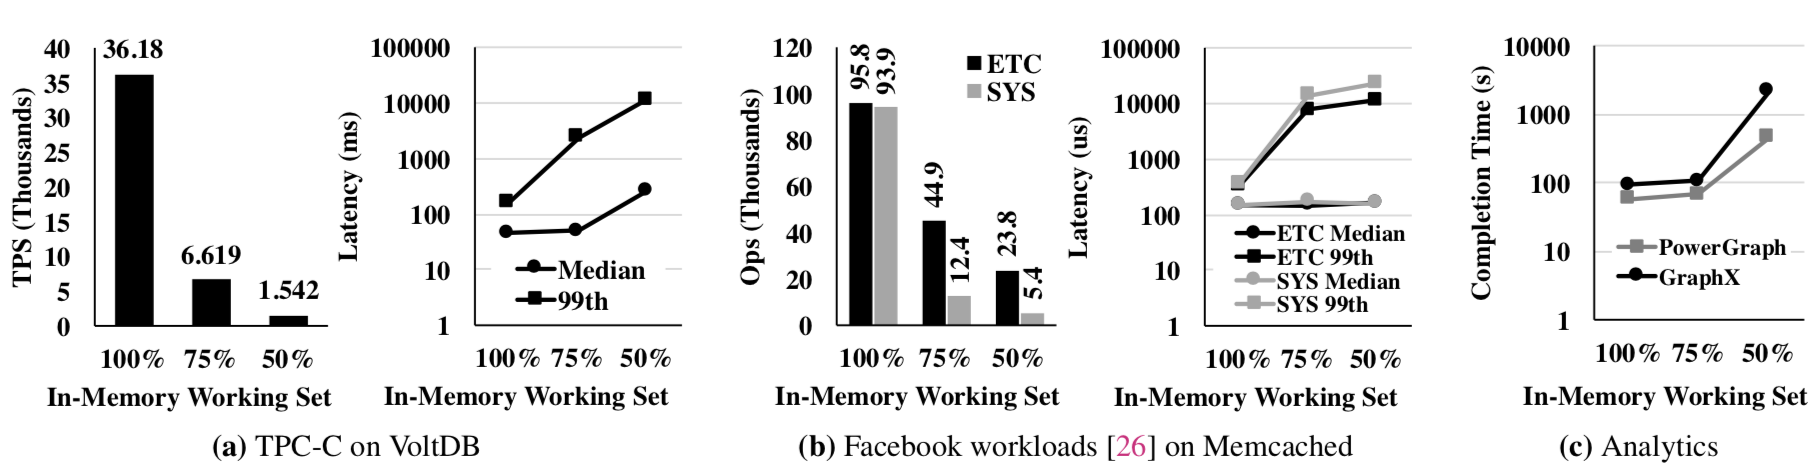
\includegraphics[scale=0.45]{Figures/memory/memory_motivation1.png}
\decoRule
\caption{在不同内存容量下应用程序的性能\cite{gu2017efficient}。}
\label{fig:memory_motivation1}
\end{figure}

为了避免由外部因素造成的性能影响,测试只关注应用程序在单机下的性能(图~\ref{fig:memory_motivation1})。
结果显示由于内存不足所导致的换页确实对应用程序产生重大的、非线性的、急速下降的性能影响。
另外,换页会导致非常明显的尾延迟现象。
以上的现象都表明,内存不足是一个非常重要的问题,进行内存分离的研究是十分有必要的。

\begin{figure}
\centering
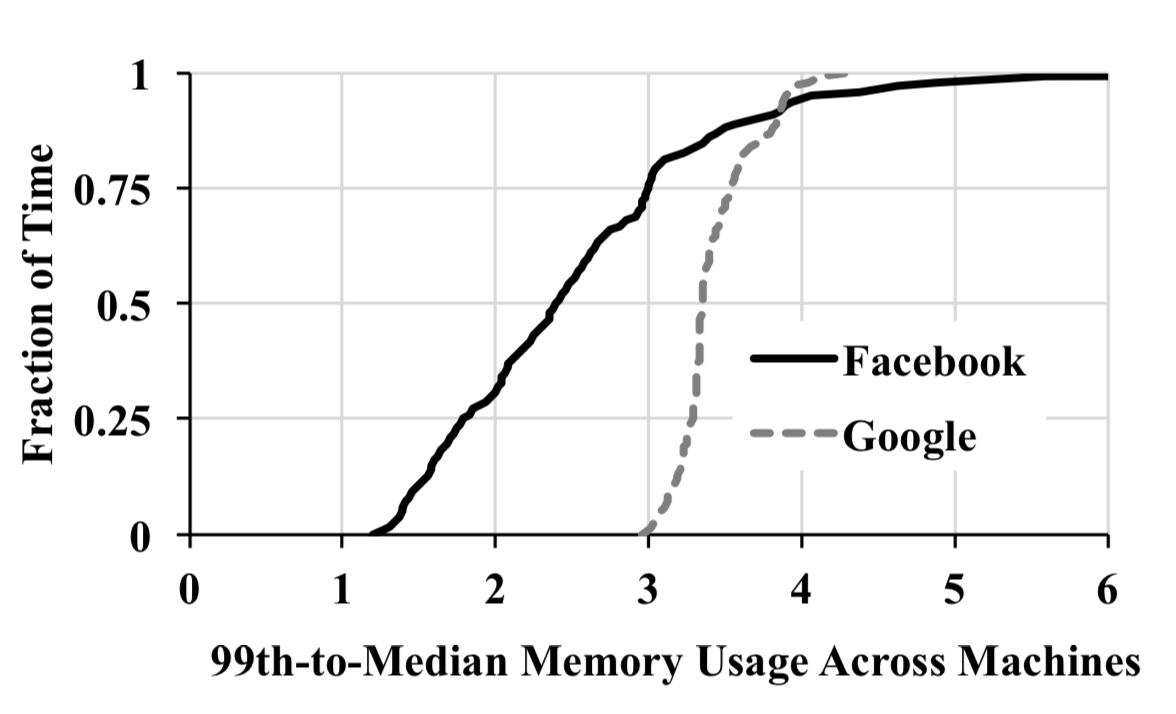
\includegraphics[scale=0.6]{Figures/memory/memory_motivation2.png}
\decoRule
\caption{Facebook和Google的两个机器集群中存在的内存使用不均衡现象\cite{gu2017efficient}。}
\label{fig:memory_motivation2}
\end{figure}

其次,不同机器中的内存使用也存在着不均衡的现象,这将导致资源浪费。
有相关的研究人员统计了Google和Facebook的两个实际运行的集群中机器内存使用情况的一些数据(图~\ref{fig:memory_motivation2})。
通过记录和计算10秒内前99\%的机器的平均内存使用率与所有机器平均使用率的比值,来表示内存使用的不均衡性。
结果显示,集群中有超过一半的内存因资源利用不均衡而导致其未被使用到的。
这样的资源利用不均衡也验证了我们的说法。


%----------------------------------------------------------------------------------------
%	SECTION 2
%----------------------------------------------------------------------------------------

\section{当前内存分离技术的研究现状}

很长一段时间以来,数据中心都在使用着一体化服务器的架构,使得大多数内存分离技术都是基于这种架构去设计并实现的,如分布式共享内存(distributed share memory)技术和远程换页(remote paging)技术。
这些方法考虑的是易用性、可行性,不需要对现有服务器架构设计进行太大的修改。

内存分离技术有多种的划分方法。
LegoOS\cite{shan2018legoos}的研究人员按照软硬件的划分将内存分离技术分成两大类,一类是硬件辅助的内存分离技术,指的是设计一些专用的小硬件来辅助和加速内存分离;
另一类是纯软件实现的内存分离技术,只需要现有的硬件设备来实现内存分离。
而INFINISWAP的研究人员则是按照实现方法来划分,将内存分离技术主要分为远程内存换页技术(Remote Memory Paging)和分布式共享内存(Distributed Shared Memory)两大类。

我们认为INFINISWAP的划分思路更加贴合内存分离的主题,我们在此基础上做一些补充,将内存分离技术可以分为如下几类:

\subsection{应用层面的分布式内存管理}

将应用部署到多台机器上,每台机器上的应用主要去管理和使用本地的内存,它们之间通过网络获取和共享各自的内存数据,这是应用层面的分布式内存管理。
其与其它内存分离技术的最大区别是,应用程序是知晓自己是处在一个分布式集群环境中的,开发人员要根据应用程序的具体情况设计内存的管理以及机器之间数据交换的方法和协议。
通常,内存密集型的一些分布式应用通常都有比较好的内存管理和交换方法,比如内存数据库、内存图计算等等,相关的系统有:DrTM\cite{wei2015fast}和Wukong\cite{shi2016fast}。

应用层面的分布式内存管理解决了单台服务器内存不足的问题,而且它灵活度高,开发人员能够根据应用程序的具体情况去设计高性能的内存管理方法和数据交换方法。
但是,这种方法也有缺点,分布式应用编程开发和调试很具有难度,而且它也并没有解决由应用程序之间内存需求不一致而导致的内存使用不均衡问题。

\subsection{远程内存换页技术}
远程内存换页技术指的是,通过网络将本地的内存页换入换出到远端机器的内存中,而不是传统那样换到本地的硬盘\cite{chen2008transparent,newhall2003nswap,flouris1999network}。
在过去,远程内存换页技术却受限于低缓的网络传输和过多的CPU的额外开销。
而现在,由于高速网络如RDMA技术的出现,远程内存换页技术的性能有了很大的提升,目前,在这一领域最先进的工作和成果是INFINISWAP\cite{gu2017efficient}。

远程换页技术对应用程序透明,单机的应用程序可以不需要进行修改便可以使用远程换页技术,因而通用性很好。
除了上面所提到的网络传输和CPU开销问题,通常的远程内存换页技术还需要中央协同器来进行页淘汰和负载均衡等工作。

\subsection{分布式共享内存}
分布式共享内存系统将集群所有机器的内存在逻辑上组织成一个全局的地址空间,供应用程序去使用,集群内部任何一台机器上的应用程序都可以对这一地址空间进行读写\cite{carter1991implementation,li1989memory,nitzberg1991distributed}。
过去的分布式共享内存技术因维护一致性而产生过多的通信开销。
现在分布式共享内存技术也使用了一些新的硬件,比如PGAS和RDMA,虽然减少了维护一致性的开销,但需要开发人员重写应用程序来使用它的接口。

分布式共享内存同样是对应用程序透明,通用性很好。
但它需要维护一致性,而且代价比较大,因而可拓展性可能会受到一定的限制。


%----------------------------------------------------------------------------------------
%	SECTION 3
%----------------------------------------------------------------------------------------

\section{案例:基于RDMA高速网络的内存分离技术——INFINISWAP}

INFINISWAP是针对RDMA高速网络设计的一个远程换页系统,通过将集群中每台机器的交换分区划分成大块去管理,适时地去收集机器中未使用的内存,并把这些内存暴露给应用程序使用。
整个过程对于应用程序来说是透明不可见的,因而应用程序不需要做任何修改。
在接下来的小节中,我们将系统设计和性能测试来对INFINISWAP系统进行介绍。

\subsection{设计目标}
INFINISWAP的主要设计目标是高效地将集群中所有机器的内存都暴露给应用程序去使用,不需要对应用程序或者操作系统做任何修改。
系统必须具备可扩展性、容错性和透明性,同时做好隔离,使用远程机器上的内存不能打扰到远程机器上应用的性能。

\begin{figure}
\centering
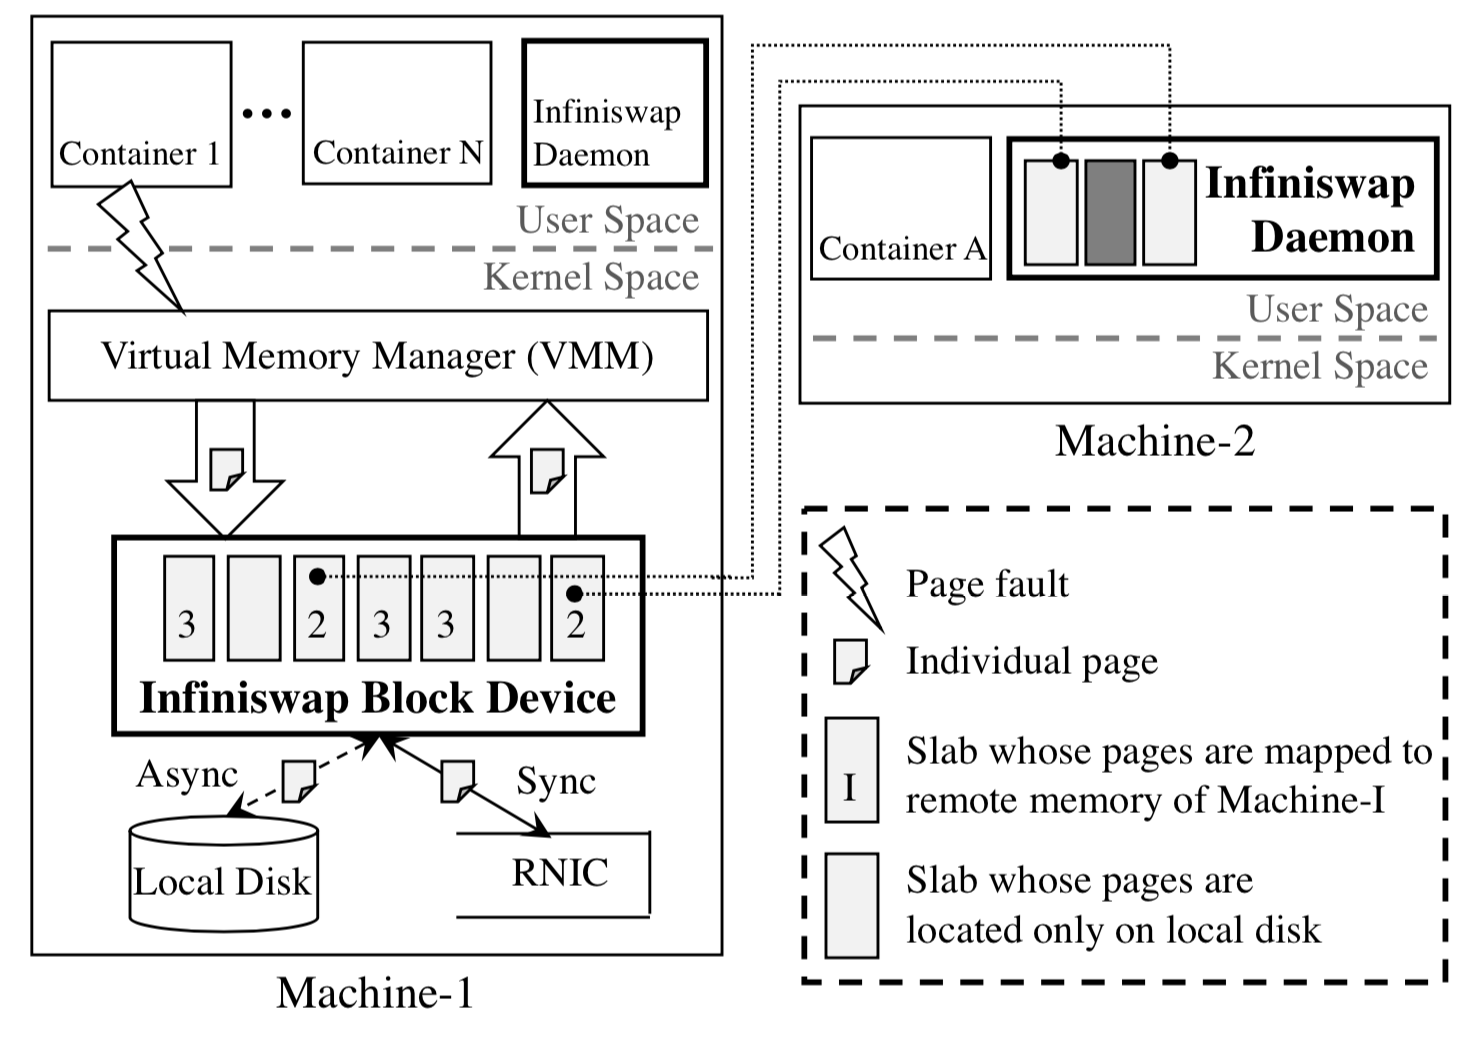
\includegraphics[scale=0.5]{Figures/memory/infiniswap_architecture.png}
\decoRule
\caption{INFINISWAP系统架构。\cite{gu2017efficient}}
\label{fig:infiniswap_architecture}
\end{figure}

\subsection{架构概述}
INFINISWAP包含了两个主要的组件——INFINISWAP块设备和INFINISWAP守护进程。
每台机器上都包含着这两个组件,因此每台机器的角色相同,从而实现了一个去中心化的系统(图~\ref{fig:infiniswap_architecture})。

\subsubsection{INFINISWAP块设备}
INFINISWAP块设备向虚拟内存管理器提供常规的块设备IO接口,让虚拟内存管理器将这个设备当成是一个交换分区。
当出现换页的时候,INFINISWAP块设备便可以透明地通过RDMA操作向其它机器中读取内存或写入内存。

INFINISWAP将每台机器上的内存地址空间划分成固定大小的大块(slab),大块是INFINISWAP内存映射和负载均衡的基本单位,它由很多内存页所组成。
以大块为单位进行内存映射处理的原因尽量减少远端机器上CPU的参与,减少对远端机器上应用程序的打扰,同时提升远程换页的速度。
当大块映射完毕之后,INFINISWAP块设备便可以通过RDMA读写操作来进行换页,换页的基本单位仍然是内存页,而不是大块。

\subsubsection{INFINISWAP守护进程}
INFINISWAP守护进程是运行在用户态的一个程序,仅仅参与控制层面(control plane)的活动。
它仅仅负责处理其它机器发过来的大块映射请求以及预先分配相应的内存空间。
真正的对数据层面(data plane)的操作则是通过RDMA请求然后由网卡去执行,并不会打扰目标机器的CPU。

\subsection{设计细节与实现}

\subsubsection{透明性和隔离性设计}
\paragraph{透明性}
INFINISWAP提供与传统块设备一样的接口和语义,应用程序不需要做任何修改便可以使用到更多的内存,它也不知道自己使用的是本地内存还是远程内存。
这样的透明性使得INFINISWAP系统具有很好的兼容性与通用性,能在现有的数据中心快速通入使用,不需要增加新的硬件。

\paragraph{隔离性}
INFINISWAP使用RDMA高速网络来传输内存页数据,不需要打扰远端CPU的执行。
对远程CPU的打扰主要在于大块的映射,但大块的大小是比内存页要大很多的,这样的一个设计也为了减少对远端机器CPU的打扰次数。

\subsubsection{容错性设计}
INFINISWAP对应用程序是透明的,应用程序认为远端机器上面的内存也是存在于本地的。
因此,INFINISWAP需要提供与应用程序只使用本地内存一样的语义,即当远端机器出现错误时,不能影响到本地应用的运行。

容错的方案是在进行RDMA远程换页的同时,异步地将内存也写入本地硬盘中做为备份。
由于写备份是异步的,并不在关键路径上,因此也不会对性能产生很大的影响。

实现这样的容错方案要处理一些边界问题,最重要的边界问题是处理\emph{read-after-write}的情况。
即当内存页已经写到远端的内存但还没有写入本地硬盘中,在这时候远端机器发生了崩溃。
如果在这同时应用程序又要读取这块内存页,块设备便需要从硬盘的写队列中读取内存页,然后返回给应用程序。

\begin{figure}
\centering
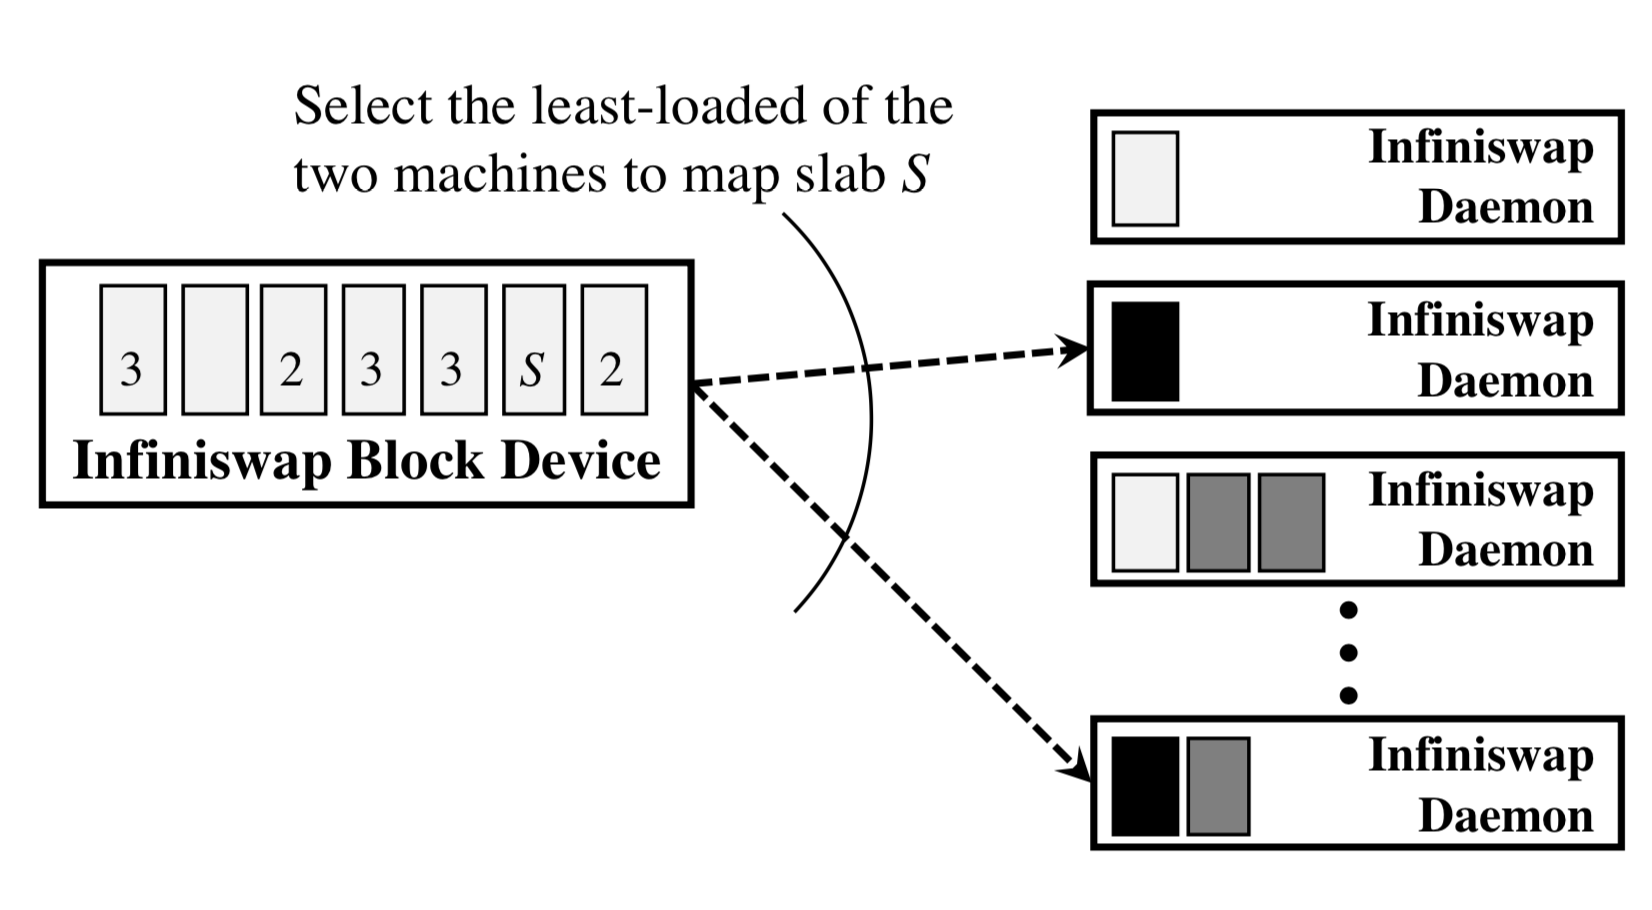
\includegraphics[scale=0.3]{Figures/memory/infiniswap_slab_mapping.png}
\decoRule
\caption{INFINISWAP块映射策略\cite{gu2017efficient}。}
\label{fig:infiniswap_slab_mapping}
\end{figure}

\begin{figure}
\centering
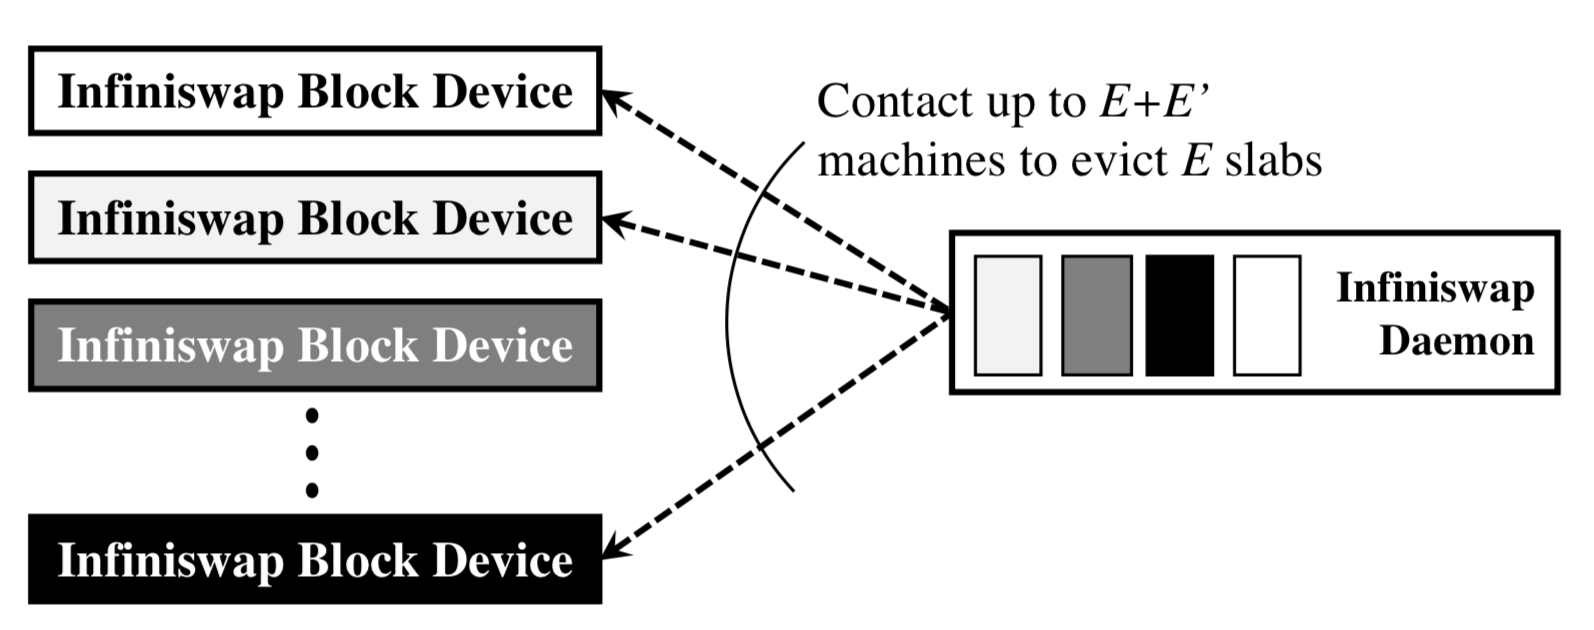
\includegraphics[scale=0.3]{Figures/memory/infiniswap_slab_eviction.png}
\decoRule
\caption{INFINISWAP块淘汰策略\cite{gu2017efficient}。}
\label{fig:infiniswap_slab_eviction}
\end{figure}

\subsubsection{可拓展性设计}
INFINISWAP并没有一个中心化的设计,避免由中央的协同器成为系统的瓶颈而导致系统不具有可拓展性。
去中心化的设计虽然能够使系统具备一定的可拓展性,但缺少中央协同器来收集全局的信息,这会带来很多问题。

其中关键的问题,如何制定好的大块映射策略来使得集群中每台机器的内存使用情况都趋于均衡。
INFINISWAP使用了\emph{power-of-choices}的技术来作为块映射以及块淘汰的策略。
比如\emph{power-of-two}的块映射策略,会先随机地选择两台远程机器,比较两台机器的内存使用情况,然后选择内存使用较少的一台机器作为目标机器来进行块映射。
类似地,块淘汰策略也是使用了\emph{power-of-choices}的方法。

\subsection{系统评测}
测试使用32台机器的集群,机器之间用56Gbps的Infiniswap网卡连接。
每台机器有2个NUMA节点和64GB的内存,每个NUMA节点有8个物理CPU,一共32个vCPU。

\begin{figure}
\centering
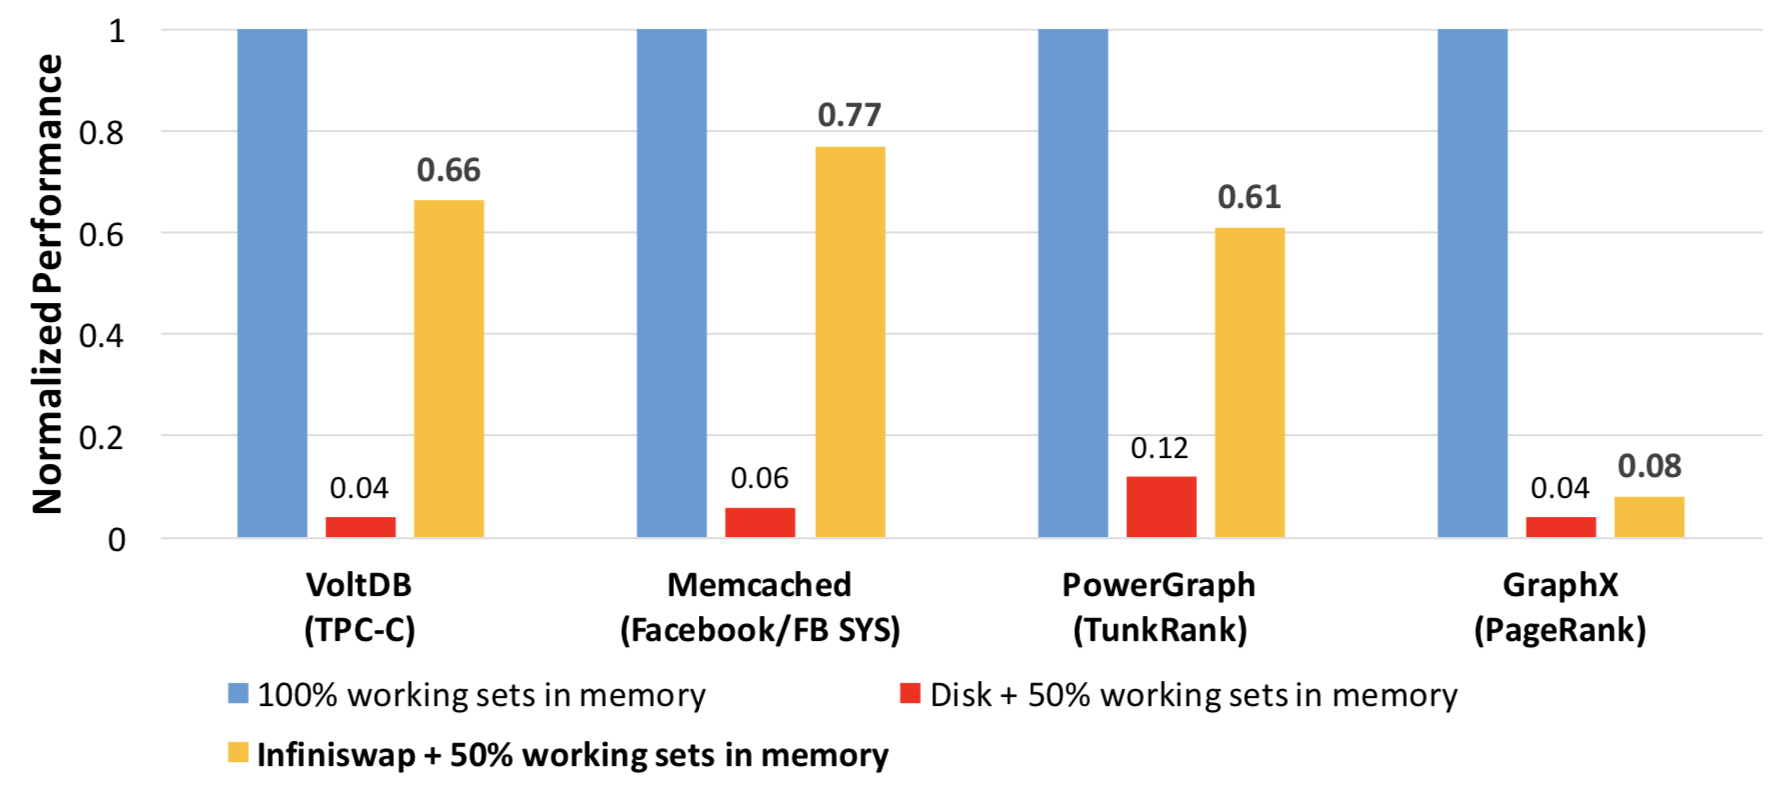
\includegraphics[scale=0.4]{Figures/memory/infiniswap_evaluation1.png}
\decoRule
\caption{应用程序的性能\cite{gu2017efficient}。}
\label{fig:infiniswap_evaluation1}
\end{figure}

\paragraph{应用程序的性能}
用于测试的应用程序有VoltDB、Memcached、PowerGraph和GraphX。
测试分别测了单机内存能满足应用程序100\%的内存需求、能满足应用程序50\%的内存需求和满足应用程序50\%的内存需求并使用INFINISWAP系统三种情况下应用程序的性能(图~\ref{fig:infiniswap_evaluation1})。
最终的测试结果表明,在单机内存只能满足应用程序50\%的内存需求时,使用INFINISWAP能将应用程序的性能提升2到16倍。

\paragraph{集群的内存使用情况}
测试创建了90个容器运行在集群上,每个容器使用不同的内存需求配置。
测试的结果显示集群的平均内存利用率从40.8\%提升到了60\%,提升了1.47倍。
而内存的不均衡现象也有所缓解(图~\ref{fig:infiniswap_evaluation2})。

\begin{figure}
\centering
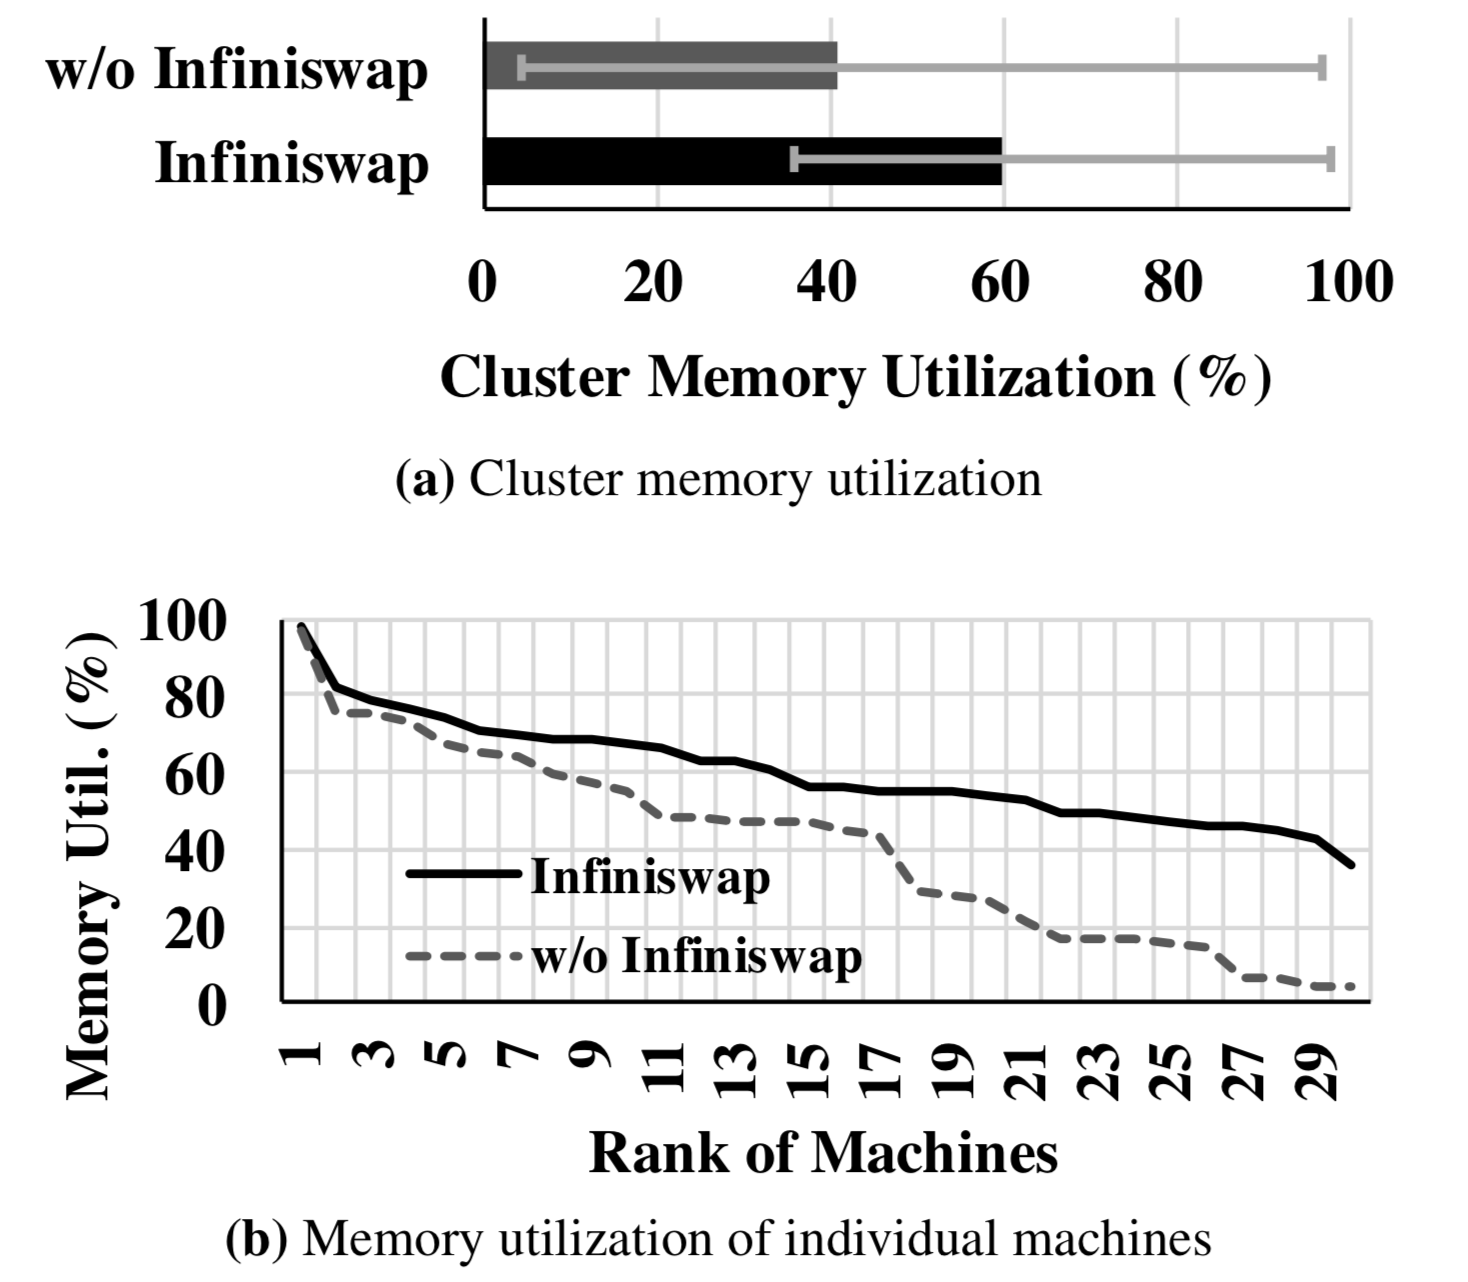
\includegraphics[scale=0.3]{Figures/memory/infiniswap_evaluation2.png}
\decoRule
\caption{集群的内存使用情况\cite{gu2017efficient}。}
\label{fig:infiniswap_evaluation2}
\end{figure}

\subsection{案例小结}
案例介绍了在内存分离领域最先进的技术INFINISWAP。
它通过RDMA技术解决了传统的远程内存换页技术所存在的网络通信慢和过多的CPU额外开销的问题。
去除了中央协同的模式,从而实现了比较好的可拓展性,还增加了容错处理。
它在一定的程度上解决了数据中心当前存在的内存不足以及内存使用不均衡问题。

%----------------------------------------------------------------------------------------
%	SECTION 4
%----------------------------------------------------------------------------------------

\section{本章小结}

本章我们探讨了内存分离这一主题,介绍了内存分离的背景、研究现状和技术案例,说明了当前数据中心存在的内存不足以及内存使用不均衡的问题,而内存分离则是解决这些问题的主流方法。

硬件的发展正不断推动着内存分离技术的发展。
实现内存分离有很多种技术方案,但无论哪种方案,都需要依靠网络来进行数据传输。
传统的内存分离技术最大的限制是网络传输速度的限制。
但现在,越来越快的一些网络技术如RDMA的出现,使得内存分离真正变得更加切实可行。

我们认为下一步的研究方向是从架构层面去思考如何去做内存分离。
内存不足以及内存使用不均衡的根本原因是一体化服务器的架构,基于这样的架构去实现的内存分离只是缓解问题,并不能从根本上去解决问题。
在后面的章节中,我们将介绍LegoOS,看看如何从根本上去解决内存的相关问题。
 
% Chapter Template

\chapter{存储分离} % Main chapter title

\label{Chapter3} % Change X to a consecutive number; for referencing this chapter elsewhere, use \ref{ChapterX}

%----------------------------------------------------------------------------------------
%	SECTION 1
%----------------------------------------------------------------------------------------
\section{资源存储的背景与发展}
资源存储策略近年来不断发展更新,其发展路线符合资源分离的理念。
%-----------------------------------
%	SUBSECTION 1
%-----------------------------------
\subsection{直连式存储}

直连式存储(Direct-attached storage, DAS)是将外置存储设备通过小型计算机系统接口(Small computer system interface, SCSI)
直接连接到服务器主机上的资源存储方式,其特征是服务器主机与存储资源一体化。
由于服务器主机与存储设备是通过物理连接,主机访问硬盘资源的速度很快。
物理连接也是最为简单直接的连接方式,实现便捷,不需要专业人员的维护,能节省维护成本。
但服务器主机的SCSI ID资源很有限,能够与之通过DAS方式连接的存储设备是有限的,所以每台服务器主机所能管理的存储资源有上限,存储资源扩展性很差。
随着业务的不断发展,当数据量达到一定规模后,一台主机的存储资源便不足以满足业务需求,此时SCSI接口数量的限制成为瓶颈。
如果采用多台服务器来分布式存储数据,由于存储空间不能跨服务器动态分配,容易造成服务器负载不均衡和资源的浪费,且难于维护。
此外,由于服务器主机与存储设备一对多的关系,使得服务器主机一旦发生故障,所有数据都将不可访问,造成较大的影响。
(图~\ref{fig:das_architecture})为DAS架构图。

\begin{figure}
\centering
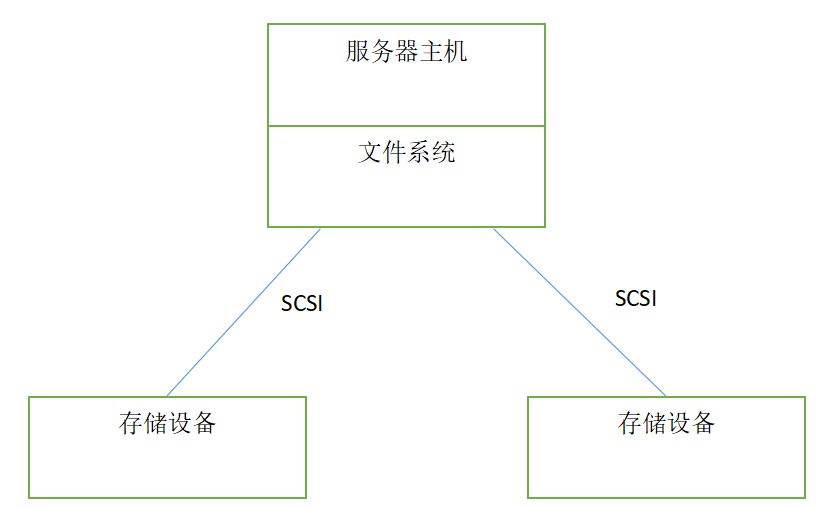
\includegraphics[scale=0.45]{Figures/storage/das_architecture.jpg}
\decoRule
\caption{DAS架构}
\label{fig:das_architecture}
\end{figure}

%-----------------------------------
%	SUBSECTION 2
%-----------------------------------
\subsection{存储区域网络}

存储区域网络(Storage Area Network, SAN)是通过网状通道(Fibre Channel, FC)交换机连接外置存储设备,建立专用于数据存储的区域网络。
在SAN模式下,服务器主机通过TCP/IP协议与存储设备通信。相比于DAS模式,SAN模式的基础是一个专用网络,可以自由地在SAN系统中添加存储设备,可扩展性大大加强。
(图~\ref{fig:san_architecture})为SAN架构图。

\begin{figure}
\centering
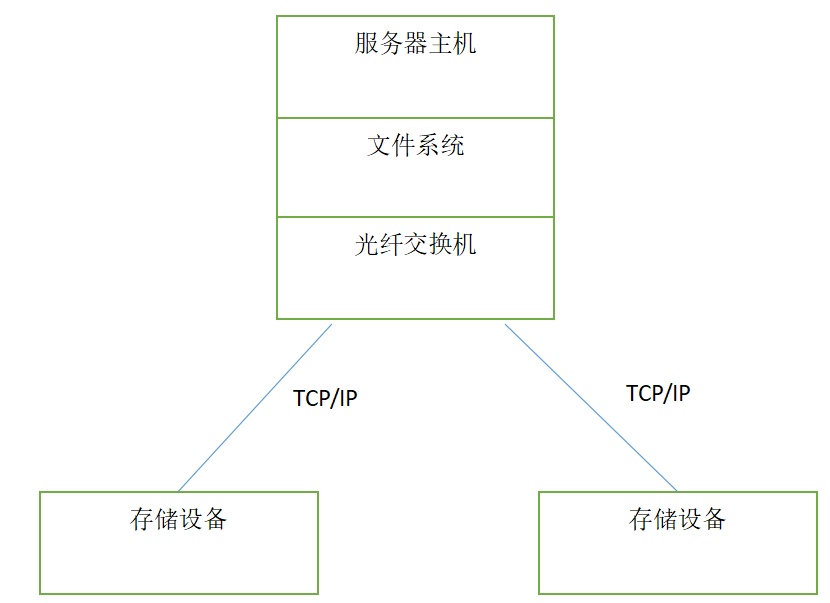
\includegraphics[scale=0.45]{Figures/storage/san_architecture.jpg}
\decoRule
\caption{SAN架构}
\label{fig:san_architecture}
\end{figure}

%-----------------------------------
%	SUBSECTION 3
%-----------------------------------
\subsection{网络附属存储}

网络附属存储(Network Attached Storage, NAS)是采用网络技术(TCP/IP, ATM, FDDI等)通过网络交换机连接存储系统和服务器主机来建立存储私网的存储模式。
NAS模式与SAN模式最大的区别在于NAS模式的文件系统位于存储设备端,其网络带宽消耗较大。
(图~\ref{fig:nas_architecture})为NAS架构图。

\begin{figure}
\centering
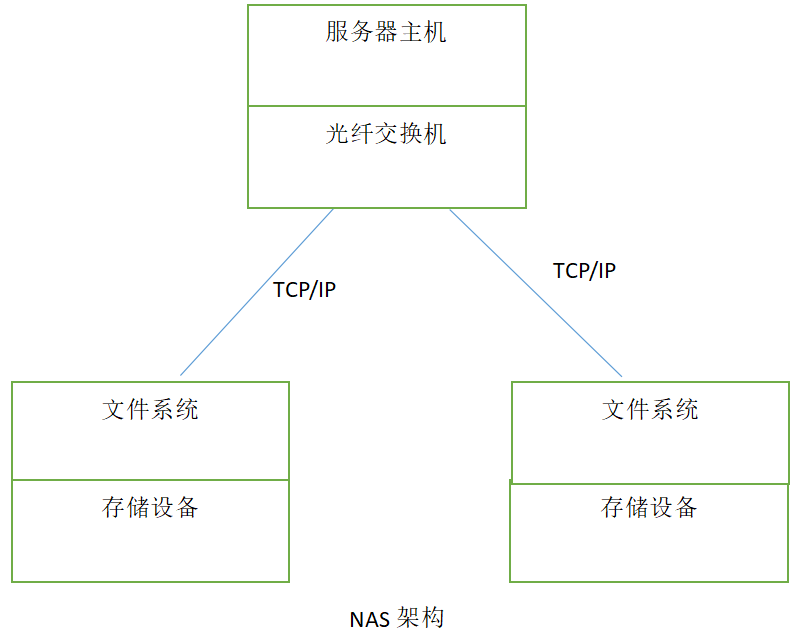
\includegraphics[scale=0.45]{Figures/storage/nas_architecture.jpg}
\decoRule
\caption{NAS架构}
\label{fig:nas_architecture}
\end{figure}

%-----------------------------------
%	SUBSECTION 4
%-----------------------------------
\subsection{发展分析}
纵观存储资源模式的发展历程,从DAS的各资源一体化,到SAN的存储资源网络化,再到NAS的文件系统网络化,存储资源的解耦程度越来越高。
这与存储资源分离(Storage Resource Disaggregation)的理念不谋而合。
存储资源分离使得存储设备从一体化的硬件中独立出去,通过控制器(Controller)转发网络信息实现与服务器主机的通信。
这样的设计能让控制器按照不同的策略动态分配存储资源的使用(如均衡化负载或集中化负载),有效缓解存储资源利用率低和存储资源不足等问题。
存储资源分离这一话题久盛不衰,许多学者在该领域从事研究工作,我们将以Klimovic等人\cite{klimovic2016flash}的工作为切入点,浅谈存储资源分离的发展和现状。

%----------------------------------------------------------------------------------------
%	SECTION 2
%----------------------------------------------------------------------------------------

\section{闪存资源分离(Flash Storage Disaggregation)}

%-----------------------------------
%	SUBSECTION 1
%-----------------------------------
\subsection{架构设计}

图~\ref{fig:d-a_flash_architecture}展示了传统的每台主机拥有一块闪存设备的架构,这意味着应用只能访问到对应的直连的闪存设备。
图~\ref{fig:dis_flash_architecture}是分离式闪存架构,其特点是闪存层(Flash Tier)从数据存储层(DataStore Tier)中解耦出来,
使得主机能够通过网络小型计算机接口(internet small computer system interface)访问所有的闪存设备,
并在闪存层增加协调管理器(coordination manager),负责选择合理的存储资源,以达到提高闪存资源利用率的目的。

\begin{figure}
\centering
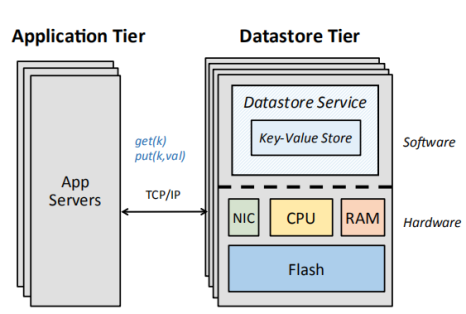
\includegraphics[scale=0.8]{Figures/storage/d-a_flash_architecture.jpg}
\decoRule
\caption{直连式闪存架构}
\label{fig:d-a_flash_architecture}
\end{figure}

\begin{figure}
\centering
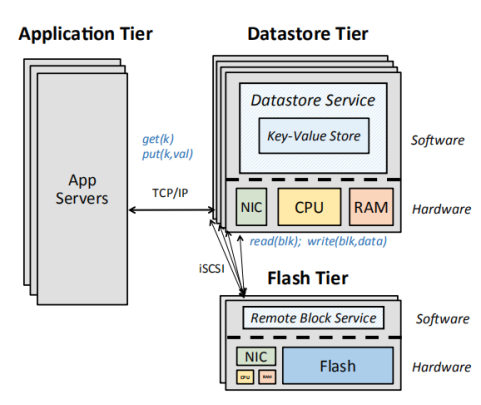
\includegraphics[scale=0.8]{Figures/storage/dis_flash_architecture.jpg}
\decoRule
\caption{分离式闪存架构}
\label{fig:dis_flash_architecture}
\end{figure}

%-----------------------------------
%	SUBSECTION 2
%-----------------------------------
\subsection{读写流程}
%-----------------------------------
%	SUBSUBSECTION 1
%-----------------------------------
\subsubsection{写流程}
iSCSI层的initiator能控制传输数据的时间,数据存储层维护一个指向协议数据单元(Protocol Data Unit, PDU)的指针。
iSCSI层对要写的数据进行包装(加入信息头等),然后由内核将PDU传输给闪存层。
其中包括的NIC和SCSI的缓存读写则取决与TCP/IP栈的实现。
%-----------------------------------
%	SUBSUBSECTION 2
%-----------------------------------
\subsubsection{读流程}
iSCSI的initiator接收到来自闪存层的包后,将使用DMA(Direct Memory Access)技术将包的数据从NIC模块转移至内核内存。
内核解析获取的包,拆离出数据内容,将之放在iSCSI的PDU。iSCSI层将PDU数据复制到SCSI缓存。
此时应用就可以从SCSI缓存中直接获取数据。

%-----------------------------------
%	SUBSECTION 3
%-----------------------------------
\subsection{性能评估}
%-----------------------------------
%	SUBSUBSECTION 1
%-----------------------------------
\subsubsection{延迟分析}
数据存储层使用RocksDB键值存储,利用mutilate负载生成器\cite{leverich2014mutilate}生成大量用户进程,进行大量的查询操作,
营造期望的每秒查询率(Queries Per Second, QPS)。图~\ref{fig:read_latency_CDF}展示了在无负载系统下,
本地闪存与远程闪存读取数据的用户延迟的累积分布函数(Cumulative Distribution Function)。
远程闪存的用户延迟显然高于本地闪存,在曲线的95\%处,远程闪存读取延迟约比本地闪存高260微秒。
由于延迟SLA在5到10毫秒左右,远远高于微秒数量级,所以远程闪存的延迟代价在可接受范围内。

\begin{figure}
\centering
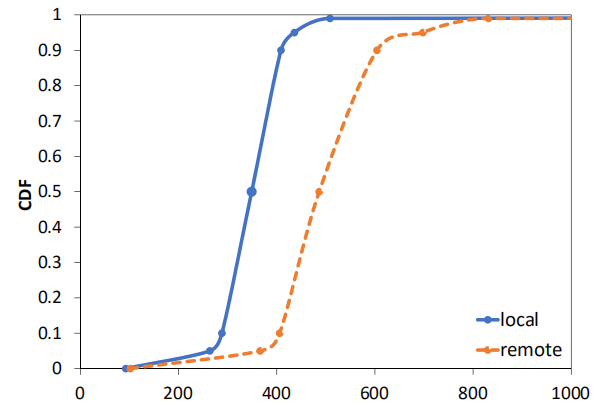
\includegraphics[scale=0.8]{Figures/storage/read_latency_CDF.jpg}
\decoRule
\caption{读操作延迟的CDF曲线}
\label{fig:read_latency_CDF}
\end{figure}

%-----------------------------------
%	SUBSUBSECTION 2
%-----------------------------------
\subsubsection{吞吐量分析}
为测试本地闪存和远程闪存的吞吐量指标,控制应用层的每秒请求率(QPS),并描绘点(QPS,延迟),图~\ref{fig:QPS_latency}展示其吞吐量性能。
由图分析,在相同延迟情况下,远程闪存吞吐量约为本地闪存的80\%。表观上,远程闪存的吞吐量受到了较严重的影响。
一方面,这是存储设备性能和资源利用率等的权衡,远程闪存的理念是牺牲了部分性能,换取更好的资源利用率。
另一方面,可以通过扩展数据存储层的CPU来补偿这些吞吐量损失。

\begin{figure}
\centering
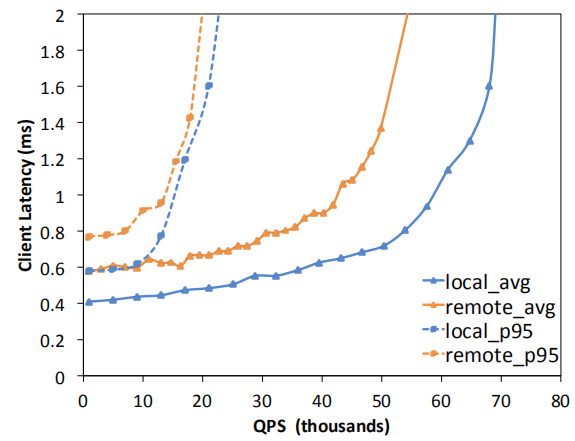
\includegraphics[scale=0.8]{Figures/storage/QPS_latency.jpg}
\decoRule
\caption{单SSDB服务器的延迟-QPS曲线}
\label{fig:QPS_latency}
\end{figure}

%-----------------------------------
%	SUBSUBSECTION 3
%-----------------------------------
\subsubsection{敏感度分析}
通过在SSDB中增加循环进程,创造不同CPU负载的环境,测试远程闪存的QPS对不同参数的曲线变化率(敏感度)。
图~\ref{fig:QPS_CPUintensity.jpg}展示了本地闪存和远程闪存在不同CPU负载下的QPS。二者在CPU负载较低的环境下,本地闪存较远程闪存有更高的QPS,
意味着远程闪存的性能受到一定影响,而在CPU处于较高负载的环境下,本地闪存与远程闪存的QPS相差无几,
意味着此时主要瓶颈不在iSCSI通讯上。同时,本地闪存的QPS受CPU负载大小的影响比远程闪存大,也就是说,远程闪存的性能表现更加稳定。


图~\ref{fig:QPS_percentage}展示了在相同请求数量下,本地闪存和远程闪存的QPS随写请求占总请求的比例变化曲线。
二者的QPS都随着写请求比例增加而增加,因为写操作的返回是异步的,其效率比读操作高。
二者的QPS差值在不同的写操作比例下差别不大,可以得出结论,读写操作所占比例对本地闪存和远程闪存性能差距影响不大。

\begin{figure}
\centering
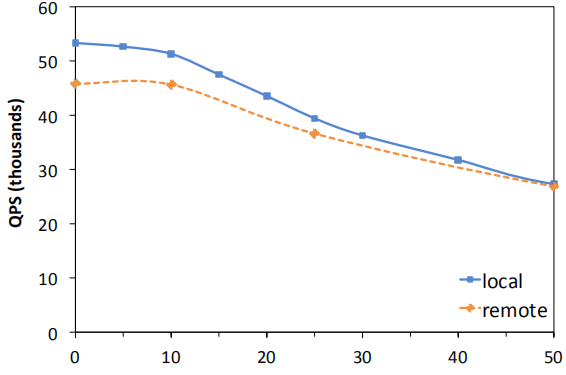
\includegraphics[scale=0.8]{Figures/storage/QPS_CPUintensity.jpg}
\decoRule
\caption{QPS随CPU负载变化曲线}
\label{fig:QPS_CPUintensity}
\end{figure}

\begin{figure}
\centering
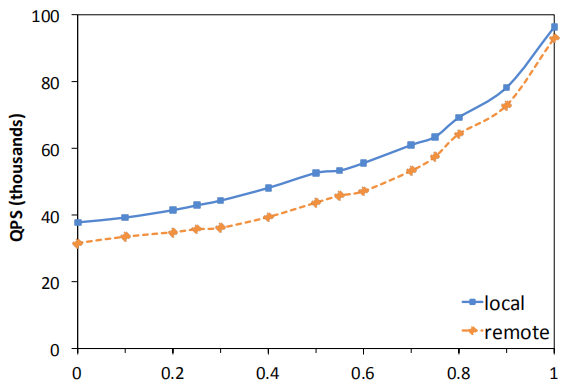
\includegraphics[scale=0.8]{Figures/storage/QPS_percentage.jpg}
\decoRule
\caption{QPS随读操作占比变化曲线}
\label{fig:QPS_percentage}
\end{figure}

%-----------------------------------
%	SUBSUBSECTION 4
%-----------------------------------
\subsubsection{多服务端性能分析}
实际情况中,机群中服务器主机与闪存时多对多的关系,所以分析多服务端共享同闪存集群的性能很有实际价值。
图~\ref{fig:2SSDB_latency_QPS}和图~\ref{fig:3SSDB_latency_QPS}分别展示两个SSDB服务器主机和三个SSDB服务器主机时,本地闪存与远程闪存的延迟-QPS曲线图。
毫无疑问,本地闪存的QPS性能始终比远程闪存更高。值得一提的是,三个SSDB环境相较于两个SSDB环境下,远程闪存的QPS性能损失代价更严重。

\begin{figure}
\centering
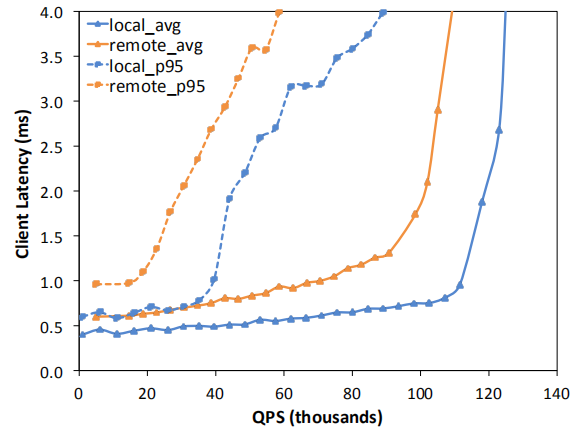
\includegraphics[scale=0.8]{Figures/storage/2SSDB_latency_QPS.jpg}
\decoRule
\caption{2个SSDB服务共享闪存下,延迟-QPS曲线}
\label{fig:2SSDB_latency_QPS}
\end{figure}

\begin{figure}
\centering
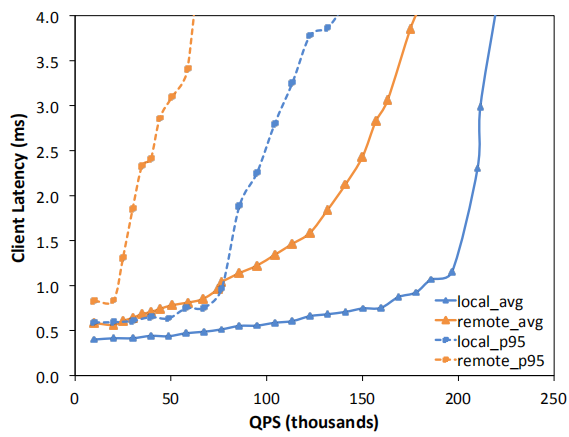
\includegraphics[scale=0.8]{Figures/storage/3SSDB_latency_QPS.jpg}
\decoRule
\caption{3个SSDB服务共享闪存下,延迟-QPS曲线}
\label{fig:3SSDB_latency_QPS}
\end{figure}

%-----------------------------------
%	SUBSECTION 4
%-----------------------------------
\subsection{存储分离适用情境分析}
通过计算直连式闪存(Direct-attached flash)和远程闪存(disaggregation flash)的主要消耗C$_{direct}$和C$_{disagg}$,对存储分离进行优势评估。
直连式闪存的消耗包括闪存读写的消耗和数据存储端CPU、RAM、NIC的消耗两部分,远程闪存则包括闪存读写的消耗,数据存储层CPU、RAM、NIC的消耗和闪存层CPU、RAM、NIC的消耗。
这些消耗的权重为目标数据与实际数据的比值,如目标QPS与实际QPS的比值。
计算而得的消耗越大,意味着其资源利用越差,反之则越好。
引入新的评估指标,消耗节约比例。
消耗节约比例含义为使用远程闪存比直连式闪存节约的消耗比例。
若消耗节约比例值为正,则表示该环境参数下远程闪存消耗比直连式闪存小;反之则远程闪存消耗更大。


图~\ref{fig:compute_storage}展示了在计算强度比例因子和存储空间比例因子分布空间下,相应的消耗节约比例。
由图例的对称性可以分析而得,闪存读写的消耗与数据存储层的CPU、RAM、NIC消耗大致相等。
在不同的情景假设下(对应图中不同的二维坐标),对资源的分配权衡也是不一样的。
若闪存资源的价值比CPU、内存低,那么服务器将倾向高闪存空间和低计算强度,对应图例的右下半边区域,该区域的消耗节约比例大于零,
意味着远程闪存消耗比直连式闪存低,则此情境下,服务器主机更适合于远程闪存。
若闪存资源的价值比CPU、内存高,那么服务器将倾向低闪存空间和高计算强度,对应图例的坐上半边区域,同理,该区域的消耗节约比例大于零,
远程闪存消耗比直连式闪存低,服务器主机更适合于远程闪存。
若闪存资源与CPU、内存资源价值相当,对应图例的对角线区域,该区域的消耗节约比例小于零,
也就是远程闪存消耗比直连式闪存高,此时服务器主机更适合直连式闪存。

\begin{figure}
\centering
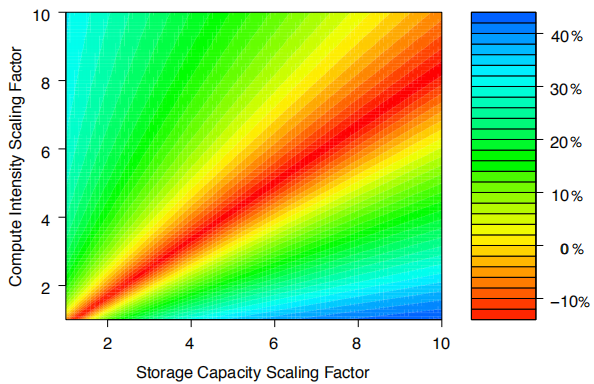
\includegraphics[scale=0.7]{Figures/storage/compute_storage.jpg}
\decoRule
\caption{消耗节约比例-计算强度比例因子-存储空间比例因子分布图}
\label{fig:compute_storage}
\end{figure}

%----------------------------------------------------------------------------------------
%	SECTION 2
%----------------------------------------------------------------------------------------

\section{本章小结}

Klimovic等人\cite{klimovic2016flash}对闪存分离策略做了充分的研究,分析了闪存分离带来的容量和资源利用率优势,也客观展示了资源分离带来的性能损失,
并提出了弥补性能损失的方法。事实上,在考虑服务器主机整体架构时,不能盲目地强调闪存分离的优势,忽略其带来的性能损失和维护成本。
分离式闪存与直连式闪存各有优劣。
更加客观的策略是,通过各类资源(如CPU,内存,闪存)的当前价值来定量计算分离式闪存带来的提升及损失孰重孰轻,进而合理取舍。
















% Chapter Template

\chapter{综合分离各类资源} % Main chapter title

\label{Chapter4} % Change X to a consecutive number; for referencing this chapter elsewhere, use \ref{ChapterX}

数据中心的规模日益扩张,对于内存的需求和存储的需求也越来越大。但是现阶段,数据中心的部署、执行、故障单元等都是一整台的物理服务器(monolithic server),这台服务器包含了运行一个程序所需要的全部硬件资源(CPU、内存、磁盘等)。在前面的两个章节中,我们讨论了内存分离和存储分离,这些技术能够部分提高数据中心对硬件资源的利用率,并且已经在现有的商业环境中应用。然而,这些技术仍然要部署到monolithic server上,无法解决monolithic serve本身的一些缺点,如缺乏弹性、单一硬件故障导致整台server失败等。

如果把所有的的硬件设备都组织为独立的组件,依靠网络进行通信,就可以完全打破monolithic server的体系结构,真正意义上实现硬件资源的分离,并且完全解决monolithic serve对弹性、异构性等支持不好的缺点。本章后面将以LegoOS为例,介绍这一思想。

%----------------------------------------------------------------------------------------
%	SECTION 1
%----------------------------------------------------------------------------------------

\section{背景介绍}

\subsection{硬件的发展}

近年来,网络的速度越来越快,甚至已接近内存总线速度的数量级。基于快速网络,分离的设备之间能够进行快速的通信,这使得硬件资源分离的思路成为可行。另一方面,硬件的功能和处理能力越发丰富。现代硬件可以整合大量以前由软件实现的逻辑,如控制器、网络协议栈等,这使得分离的硬件组件能够高效的进行本地管理,而不依赖CPU资源和复杂的软件逻辑。

\subsection{单一硬件资源的分离}

目前已有很多针对单一硬件资源分离的研究。例如,针对内存资源,有基于RDMA的远程换页系统INFINISWAP\parencite{gu2017efficient},可以透明的把本地计算机的内存交换到集群中另一台计算机的内存上;针对存储资源,有Flash storage disaggregation\parencite{klimovic2016flash},把闪存层从数据存储层解耦出来集中管理,使得网络中的主机可以通过统一的接口读写闪存设备。

\subsection{系统层面的分离}

现有的操作系统大多以单台机器为管理单元,并假设所有硬件资源都位于本地。这种体系结构从根本上不利于硬件资源的分离。比较好的方法是从底层按照分离的思路重新设计操作系统,这样不仅简化了抽象层,还可以打破单机操作系统管理分布式硬件的语义隔离,能更好地适应分离的硬件结构。但是,重新设计一套系统架构,并且能够较好的对分布式资源进行管理,是非常困难的。不过,目前已存在一些尝试,如Helios\parencite{nightingale2009helios}在NUMA架构的异构核心上构建了一组satellite kernel。

%----------------------------------------------------------------------------------------
%	SECTION 2
%----------------------------------------------------------------------------------------

\section{相关研究}

\subsection{多机分布式计算框架}

随着需要分析处理的数据量不断增大,单台机器无法完成海量数据的计算和存储。分布式计算在此背景下产生,其主要思想是把数据和计算任务分配到多台机器上,每台机器只需承担很少的任务。这其中涉及到集群管理、消息通信、任务分发等复杂的逻辑。一些分布式计算框架,如Hadoop、Spark等的出现简化了用户的使用,用户只需编写自己的业务逻辑,底层全部交给框架处理。

这带来了很多好处,如资源被分摊到了每台机器上,单台机器的故障不会使任务彻底中断;一个良好的调度策略能够根据每台机器的性能和负载合理分配任务,尽可能最大化利用每台机器的资源;集群中的机器可以根据需要随时添加或移除;等。但是,分布式计算集群的调度单位是一整台机器,粒度很粗,无法解决单台机器内部的问题,如单台机器各硬件负载不均衡导致资源浪费。

\subsection{巨型虚拟机}

针对多机的资源利用,还有一种分布式操作系统的方案。其原理把每台机器的硬件资源综合在一起(例如,综合所有机器实现分布式共享内存),对外则表现为一个巨型的虚拟机。结合调度,单一的任务也能够利用到不同机器的资源,提高了硬件资源的整体利用率。但是,这种设计对节点间的通信要求较高,同时调度的策略和性能也会带来很大影响。

Amoeba\parencite{tanenbaum1991amoeba}是一个例子,它在每台机器的每个处理器核上运行一个microkernel,实现了一个共享的处理器池,为每个用户动态分配处理器资源。相比于多机分布式计算,Amoeba使资源调度的粒度减小到了进程的级别。

\subsection{弹性计算}

现在,很多云服务商都提供弹性计算服务。用户可以根据自己对资源的使用需求,灵活配置和购买。云服务商在后台管理着大量机器,将物理资源(如CPU、内存、存储、带宽等)虚拟化,并在多台机器上打通。用户对资源的使用常常是突发的,这样大多数时间物理资源是空闲的,服务商可以暂时把资源分配给其他用户。依靠资源的虚拟化和分解,实现了所有资源的按需分配,使硬件资源得到了尽可能高的利用效率。

%----------------------------------------------------------------------------------------
%	SECTION 3
%----------------------------------------------------------------------------------------

\section{案例分析:LegoOS}

\subsection{设计目标}

多年来,monolithic server一直是数据中心的部署和操作单元,但这种以单台服务器未中心的架构有几个重要的问题:
\begin{itemize}
\item 资源利用率低:由于对于同一个任务必须从同一台机器分配CPU和内存,而程序对资源的利用是不平衡的,导致硬件利用率整体不高。
\item 硬件弹性差:一旦完成单台服务器的组装,就很难添加或删除硬件组件。
\item 故障范围大:单台服务器由很多硬件组件组成,任何一个组件的损坏都会使得服务器无法工作。
\item 对异构硬件支持不好:组成单台服务器的硬件之间往往紧密的耦合,一些专用的、非传统的硬件往往难以和其他硬件组件结合。
\end{itemize}

针对以上问题,提出了一种新的硬件资源分解的架构,能够使各硬件组件完全拆分开,并在此基础上构建了LegoOS系统。

\subsection{整体架构}

\begin{figure}[h]
\centering
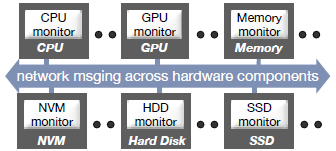
\includegraphics[scale=1.00]{Figures/legoos/splitkernel.png}
\decoRule
\caption{Splitkernel Archiecture}
\label{fig:legoos_archiecture}
\end{figure}

Splitkernel模型分解了传统操作系统的功能,并将这些功能转入松散耦合的硬件组件的监视器中。每个监视器在本地运行,管理着自己的硬件组件,并仅在需要时通过网络以显式的消息传递与其他组件通信。

LegoOS是基于splitkernel模型构建的一个专为硬件资源分解的操作系统。它将操作系统的功能分为了三类监视器:处理器监视器、内存监视器和存储监视器。除了处理器,每个硬件组件期望有一个硬件控制器,可以执行监视器的逻辑。LegoOS有全局的资源管理器GPM、GMM和GSM,用来粗粒度的分配处理器、内存和存储资源。细粒度的分配由各自的监视器决定。

\subsection{具体实现}

LegoOS在设计上针对三种硬件组件:处理器、内存、存储,分别称之为pComponent、mComponent、sComponent。在接口方面,LegoOS暴露给用户的是一组vNode。每个vNode有自己独立的IP,可以运行多个pComponent、mComponent、sComponent。LegoOS确保每个vNode的资源相互之间完全隔离。LegoOS实现了大多数的Linux system call接口,使得大多数程序可以未修改的在LegoOS的一组vNode上运行。

\subsubsection{处理器管理}

\begin{figure}[h]
\centering
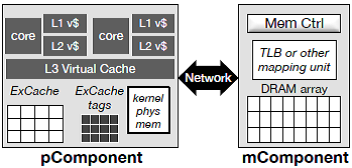
\includegraphics[scale=1.00]{Figures/legoos/pcomponent_mcomponent.png}
\decoRule
\caption{LegoOS pComponent and mComponent Archiecture}
\label{fig:legoos_archiecture}
\end{figure}

pComponent专门管理处理器内核。它使用了针对数据中心程序的一个简单的调度模型。每个pComponent为内核线程保留少量的核心,然后分配其他的核心给用户线程。当用户启动一个新进程时,由全局的GPM选择一个托管线程数最少的pComponent,然后这个pComponent为用户线程分配CPU核心,并且尽量减少线程调度和内核抢占以提高性能(例如,不使用中断而是用轮询处理网络请求,因为网络延迟在LegoOS中很低)。因为全局GPM的存在,调度策略的着重于最小化上下文切换的开销,而不是单个线程的核心利用率。

pComponent完全不需要地址映射,mmu和TLB等全部由mComponent维护。为了性能,在本地pComponent仍持有少量的(如4GB)内存缓存,称为ExCache,位于处理器的Last-Level Cache(LLC)之下,而剩余的大量内存通过网络从mComponent访问。每个ExCache line有一个虚拟地址的tag和两个标记位(P,R/W),由软件设置、硬件检查。当ExCache miss时,LegoOS通过网络从对应的mComponent中取回数据填入ExCache line中。ExCache miss的处理甚至可以完全由硬件实现以获得最高的效率。

ExCache冷不命中会产生很多访问mComponent的请求,带来了较大的性能开销。为此有一个简单的优化。注意到匿名内存的初始内容为零,因此可以直接在ExCache中分配这些line,直到这个ExCache line被flush,才首次发送到mComponent中。在设计上LegoOS的pComponent不共享内存,因此不会产生竞争。

\subsubsection{内存管理}

\begin{figure}[h]
\centering
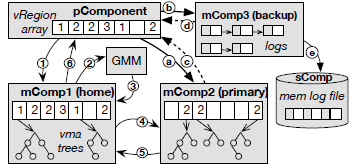
\includegraphics[scale=1.00]{Figures/legoos/memory_management.png}
\decoRule
\caption{LegoOS Distributed Memory Management}
\label{fig:legoos_memory_management}
\end{figure}

mComponent管理虚拟内存和物理内存,包括它们的分配、回收和映射。为了最小化网络通信,这里采用了两级的内存管理。在high level,把虚拟地址空间粗粒度的划分为了固定大小的vRegions,每个已被分配的vRegion都被一个mComponent管理。在low level,mComponent记录了每个vRegion上分配给用户的vma树。一个用户进程的虚拟地址空间可以跨越多个mComponent。用户进程还有一个home mComponent,它只是记录进程的每个vRegion分别由哪个mComponnet在管理(vRegion array),以及每个vRegion内的剩余未分配空间。

当用户程序申请虚拟内存空间时,pComponent把相关的请求转发给进程的home mComponent。home mComponent会查询vRegion array,寻找一个合适的vRegion,然后把请求再转发给对应的mComponent,由它来为用户分配vma。如果可用虚拟内存空间不足,home mComponent还会向全局的内存资源管理器GMM申请一个新的vRegion并把请求转发到另一个mComponent。(实现上为了快速访问,pComponent也缓存了一份vRegion array)

考虑到内存故障的可能性与影响更大,LegoOS对mComponent提供了可靠性保证:使用primary mComponent和backup mComponent。当pComponent刷新ExCache时,消息被同时发往primary mComponnet和对应的backup mComponent。其中primary mComponent维护内存数据和元数据,backup mComponent在后台把内存操作写入由sComponent管理的append-only log中,这样可以在失败时通过log恢复内存内容。

\subsubsection{存储管理}

LegoOS在sComponent上实现存储功能。类似于NFS,存储服务器采用无状态的设计,并通过vNode抽象后暴露给用户。用户可以通过标准POSIX api操作vNode上的挂载点,从而访问存储系统。

由于sComponent的内部内存有限,LegoOS在mComponent上放置存储缓冲区。当用户通过系统调用访问文件时,抽象层把请求的文件完整路径、偏移量和大小转发给mComponent,mComponent查找缓冲区,并在需要时从sComponent获取缺失的数据以及将文件数据sync到sComponent中。

\subsection{测试评估}

由于并没有真正的资源分解硬件,硬件组件实际由服务器模拟而来,通过限制可用的资源使其符合各个componnet的设定。

\begin{figure}[h]
\centering
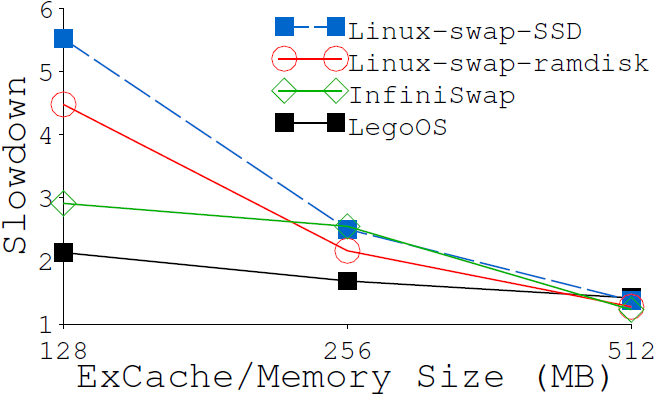
\includegraphics[scale=0.50]{Figures/legoos/tensorflow_perf.png}
\decoRule
\caption{TensorFlow Performance}
\label{fig:tensorflow_perf}
\end{figure}

\begin{figure}[h]
\centering
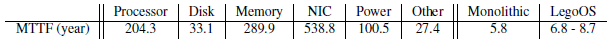
\includegraphics[scale=0.75]{Figures/legoos/failure_analysis.png}
\decoRule
\caption{Mean Time To Failure Analysis}
\label{fig:failure_analysis}
\end{figure}

\begin{itemize}
\item TensorFlow:在LegoOS上运行一个未修改的TesorFlow程序,其working set是0.9GB,为它分配了1个pComponent、1个mComponent、1个sComponent。测试的基准是一个无限内存的Linux系统。在有限的内存下,LegoOS的Slowdown显著低于其他的swap方案的OS。
\item 故障分析:通过收集到的各硬件的平均无故障运行时间(MTTF),可以分别计算出monolithic server和LegoOS的MTTF。由于LegoOS的组件完全分离,并且资源利用率接近100\%(传统的monolithic server集群的资源利用率只有大约50\%),使得MTTF提高了17\%-49\%。
\end{itemize}

%----------------------------------------------------------------------------------------
%	SECTION 3
%----------------------------------------------------------------------------------------

\section{本章小结}

本章主要介绍了一些综合分离各类资源的方案,如传统的多机分布式计算、巨型虚拟机,以及在云服务商大规模应用的弹性计算。这些方案从不同的技术原理、以不同的粒度实现了一定的资源分离,提高了一定的资源利用率。硬件的发展,为软件的实现提供了新的可能,使得可以跳出现有框架的限制,去尝试一些颠覆性思路。最后讨论了LegoOS,以一种全新的架构完全分离了各个硬件组件,从根本上解决了monolithic server的缺陷。
 
%\chapter{总结} % Main chapter title

\label{Chapter5} % Change X to a consecutive number; for referencing this chapter elsewhere, use \ref{ChapterX}

章节\ref{Chapter1}从计算力发展与计算需求变化的角度,阐述了大规模计算对硬件资源
利用率提出的新要求,介绍了硬件资源分离这一研究方向的背景。

章节\ref{Chapter2}对内存资源分离技术进行了介绍。
我们介绍了内存资源分离的问题现状与提高内存资源利用率的常见分离技术设计与实现,
并以INFINITESWAP为案例,详细介绍了在高速网络下,内存资源分离的挑战、解决方案与
性能评估。

章节\ref{Chapter3}对存储资源分离技术进行了介绍。
我们介绍了存储技术的发展,在当前面临的挑战,介绍并对比了目前常见的解决方案。
以当前普遍使用的闪存介质为例,我们详细介绍了其中一种解决方案的设计挑战、设计细
节与性能评估。

章节\ref{Chapter4}对系统性的硬件资源分离技术进行了介绍,本节不再关注特定一种资
源,而是如何在统一的框架下将各类资源进行分离,从而提高整体的利用率。
我们介绍了多种实现这一目标的技术与系统,并以LegoOS为案例,详细介绍分析了其设计
原则与实现细节。

\textbf{硬件资源分离是未来趋势。}
目前,处理器的摩尔定律正面临失效的挑战,而随着工业物联网、区块链技术与人工智能
的普及,逐渐增加并复杂化的计算需求却对计算资源提出越来越高的要求。
另一方面,大规模数据中心中存在的资源利用率不理想问题与扩展性挑战却使得计算能力
并不能有效地转化为完成的计算任务。
为解决这一矛盾,最直接有效地方法便是将硬件资源结偶,不局限与单台机器,允许其被
动态地分配给不同的计算任务,及所谓的硬件资源分离。

\textbf{单纯的将硬件资源分离管理并不足够。}
随着硬件资源间的结偶与新硬件技术的发展,以往的假设与顾虑往往不复存在,我们需要
针对性的进行分析与重新设计,才能真正地发掘出硬件资源分离的潜力。
同时,为了将资源发挥到极致,在分离基础上,我们也应该进一步考虑如何设计方案,使
上层软件能够更好地利用新的硬件资源模型。

我们相信并期待硬件资源分离技术被广泛使用在大型数据中心,产生重要的影响。 


%----------------------------------------------------------------------------------------
%	THESIS CONTENT - APPENDICES
%----------------------------------------------------------------------------------------

%\appendix % Cue to tell LaTeX that the following "chapters" are Appendices

% Include the appendices of the thesis as separate files from the Appendices folder
% Uncomment the lines as you write the Appendices

%% Appendix A

\chapter{Frequently Asked Questions} % Main appendix title

\label{AppendixA} % For referencing this appendix elsewhere, use \ref{AppendixA}

\section{How do I change the colors of links?}

The color of links can be changed to your liking using:

{\small\verb!\hypersetup{urlcolor=red}!}, or

{\small\verb!\hypersetup{citecolor=green}!}, or

{\small\verb!\hypersetup{allcolor=blue}!}.

\noindent If you want to completely hide the links, you can use:

{\small\verb!\hypersetup{allcolors=.}!}, or even better: 

{\small\verb!\hypersetup{hidelinks}!}.

\noindent If you want to have obvious links in the PDF but not the printed text, use:

{\small\verb!\hypersetup{colorlinks=false}!}.

%\include{Appendices/AppendixB}
%\include{Appendices/AppendixC}

%----------------------------------------------------------------------------------------
%	BIBLIOGRAPHY
%----------------------------------------------------------------------------------------

\printbibliography[heading=bibintoc]

%----------------------------------------------------------------------------------------

\end{document}  
